% Options for packages loaded elsewhere
\PassOptionsToPackage{unicode}{hyperref}
\PassOptionsToPackage{hyphens}{url}
\PassOptionsToPackage{dvipsnames,svgnames,x11names}{xcolor}
%
\documentclass[
  letterpaper,
  DIV=11,
  numbers=noendperiod]{scrartcl}

\usepackage{amsmath,amssymb}
\usepackage{iftex}
\ifPDFTeX
  \usepackage[T1]{fontenc}
  \usepackage[utf8]{inputenc}
  \usepackage{textcomp} % provide euro and other symbols
\else % if luatex or xetex
  \usepackage{unicode-math}
  \defaultfontfeatures{Scale=MatchLowercase}
  \defaultfontfeatures[\rmfamily]{Ligatures=TeX,Scale=1}
\fi
\usepackage{lmodern}
\ifPDFTeX\else  
    % xetex/luatex font selection
\fi
% Use upquote if available, for straight quotes in verbatim environments
\IfFileExists{upquote.sty}{\usepackage{upquote}}{}
\IfFileExists{microtype.sty}{% use microtype if available
  \usepackage[]{microtype}
  \UseMicrotypeSet[protrusion]{basicmath} % disable protrusion for tt fonts
}{}
\makeatletter
\@ifundefined{KOMAClassName}{% if non-KOMA class
  \IfFileExists{parskip.sty}{%
    \usepackage{parskip}
  }{% else
    \setlength{\parindent}{0pt}
    \setlength{\parskip}{6pt plus 2pt minus 1pt}}
}{% if KOMA class
  \KOMAoptions{parskip=half}}
\makeatother
\usepackage{xcolor}
\setlength{\emergencystretch}{3em} % prevent overfull lines
\setcounter{secnumdepth}{5}
% Make \paragraph and \subparagraph free-standing
\makeatletter
\ifx\paragraph\undefined\else
  \let\oldparagraph\paragraph
  \renewcommand{\paragraph}{
    \@ifstar
      \xxxParagraphStar
      \xxxParagraphNoStar
  }
  \newcommand{\xxxParagraphStar}[1]{\oldparagraph*{#1}\mbox{}}
  \newcommand{\xxxParagraphNoStar}[1]{\oldparagraph{#1}\mbox{}}
\fi
\ifx\subparagraph\undefined\else
  \let\oldsubparagraph\subparagraph
  \renewcommand{\subparagraph}{
    \@ifstar
      \xxxSubParagraphStar
      \xxxSubParagraphNoStar
  }
  \newcommand{\xxxSubParagraphStar}[1]{\oldsubparagraph*{#1}\mbox{}}
  \newcommand{\xxxSubParagraphNoStar}[1]{\oldsubparagraph{#1}\mbox{}}
\fi
\makeatother


\providecommand{\tightlist}{%
  \setlength{\itemsep}{0pt}\setlength{\parskip}{0pt}}\usepackage{longtable,booktabs,array}
\usepackage{calc} % for calculating minipage widths
% Correct order of tables after \paragraph or \subparagraph
\usepackage{etoolbox}
\makeatletter
\patchcmd\longtable{\par}{\if@noskipsec\mbox{}\fi\par}{}{}
\makeatother
% Allow footnotes in longtable head/foot
\IfFileExists{footnotehyper.sty}{\usepackage{footnotehyper}}{\usepackage{footnote}}
\makesavenoteenv{longtable}
\usepackage{graphicx}
\makeatletter
\newsavebox\pandoc@box
\newcommand*\pandocbounded[1]{% scales image to fit in text height/width
  \sbox\pandoc@box{#1}%
  \Gscale@div\@tempa{\textheight}{\dimexpr\ht\pandoc@box+\dp\pandoc@box\relax}%
  \Gscale@div\@tempb{\linewidth}{\wd\pandoc@box}%
  \ifdim\@tempb\p@<\@tempa\p@\let\@tempa\@tempb\fi% select the smaller of both
  \ifdim\@tempa\p@<\p@\scalebox{\@tempa}{\usebox\pandoc@box}%
  \else\usebox{\pandoc@box}%
  \fi%
}
% Set default figure placement to htbp
\def\fps@figure{htbp}
\makeatother
% definitions for citeproc citations
\NewDocumentCommand\citeproctext{}{}
\NewDocumentCommand\citeproc{mm}{%
  \begingroup\def\citeproctext{#2}\cite{#1}\endgroup}
\makeatletter
 % allow citations to break across lines
 \let\@cite@ofmt\@firstofone
 % avoid brackets around text for \cite:
 \def\@biblabel#1{}
 \def\@cite#1#2{{#1\if@tempswa , #2\fi}}
\makeatother
\newlength{\cslhangindent}
\setlength{\cslhangindent}{1.5em}
\newlength{\csllabelwidth}
\setlength{\csllabelwidth}{3em}
\newenvironment{CSLReferences}[2] % #1 hanging-indent, #2 entry-spacing
 {\begin{list}{}{%
  \setlength{\itemindent}{0pt}
  \setlength{\leftmargin}{0pt}
  \setlength{\parsep}{0pt}
  % turn on hanging indent if param 1 is 1
  \ifodd #1
   \setlength{\leftmargin}{\cslhangindent}
   \setlength{\itemindent}{-1\cslhangindent}
  \fi
  % set entry spacing
  \setlength{\itemsep}{#2\baselineskip}}}
 {\end{list}}
\usepackage{calc}
\newcommand{\CSLBlock}[1]{\hfill\break\parbox[t]{\linewidth}{\strut\ignorespaces#1\strut}}
\newcommand{\CSLLeftMargin}[1]{\parbox[t]{\csllabelwidth}{\strut#1\strut}}
\newcommand{\CSLRightInline}[1]{\parbox[t]{\linewidth - \csllabelwidth}{\strut#1\strut}}
\newcommand{\CSLIndent}[1]{\hspace{\cslhangindent}#1}

\usepackage{cancel}
\addtokomafont{disposition}{\rmfamily}
\KOMAoption{captions}{tableheading}
\makeatletter
\@ifpackageloaded{caption}{}{\usepackage{caption}}
\AtBeginDocument{%
\ifdefined\contentsname
  \renewcommand*\contentsname{Table of contents}
\else
  \newcommand\contentsname{Table of contents}
\fi
\ifdefined\listfigurename
  \renewcommand*\listfigurename{List of Figures}
\else
  \newcommand\listfigurename{List of Figures}
\fi
\ifdefined\listtablename
  \renewcommand*\listtablename{List of Tables}
\else
  \newcommand\listtablename{List of Tables}
\fi
\ifdefined\figurename
  \renewcommand*\figurename{Figure}
\else
  \newcommand\figurename{Figure}
\fi
\ifdefined\tablename
  \renewcommand*\tablename{Table}
\else
  \newcommand\tablename{Table}
\fi
}
\@ifpackageloaded{float}{}{\usepackage{float}}
\floatstyle{ruled}
\@ifundefined{c@chapter}{\newfloat{codelisting}{h}{lop}}{\newfloat{codelisting}{h}{lop}[chapter]}
\floatname{codelisting}{Listing}
\newcommand*\listoflistings{\listof{codelisting}{List of Listings}}
\usepackage{amsthm}
\theoremstyle{plain}
\newtheorem{proposition}{Proposition}[section]
\theoremstyle{plain}
\newtheorem{lemma}{Lemma}[section]
\theoremstyle{remark}
\AtBeginDocument{\renewcommand*{\proofname}{Proof}}
\newtheorem*{remark}{Remark}
\newtheorem*{solution}{Solution}
\newtheorem{refremark}{Remark}[section]
\newtheorem{refsolution}{Solution}[section]
\makeatother
\makeatletter
\makeatother
\makeatletter
\@ifpackageloaded{caption}{}{\usepackage{caption}}
\@ifpackageloaded{subcaption}{}{\usepackage{subcaption}}
\makeatother

\usepackage{bookmark}

\IfFileExists{xurl.sty}{\usepackage{xurl}}{} % add URL line breaks if available
\urlstyle{same} % disable monospaced font for URLs
\hypersetup{
  pdftitle={The behavioral effects of index insurance in fisheries},
  pdfauthor={Nathaniel Grimes; Christopher Costello; Andrew J. Plantinga},
  pdfkeywords={Index Insurance, Moral Hazard, Fisheries, Conservation},
  colorlinks=true,
  linkcolor={blue},
  filecolor={Maroon},
  citecolor={Blue},
  urlcolor={Blue},
  pdfcreator={LaTeX via pandoc}}


\title{The behavioral effects of index insurance in fisheries}
\usepackage{etoolbox}
\makeatletter
\providecommand{\subtitle}[1]{% add subtitle to \maketitle
  \apptocmd{\@title}{\par {\large #1 \par}}{}{}
}
\makeatother
\subtitle{Working Paper Draft \emph{Not For Circulation}}
\author{Nathaniel Grimes \and Christopher Costello \and Andrew J.
Plantinga}
\date{2025-06-25}

\begin{document}
\maketitle
\begin{abstract}
Fisheries are vulnerable to environmental shocks that impact stock
health and fisher income. Index insurance is a promising financial tool
to protect fishers from environmental risk. However, insurance may
change fisher's behavior in ways that exacerbate problems from
overfishing. We provide the first theoretical application of index
insurance on fisher's behavior change to predict if index insurance will
incentivize higher or lower harvests in unregulated settings. The
direction of harvest changes depends primarily on: the ability for
fishers to mitigate production risk, the correlation between sources of
risk, and the type of risk protected by the insurance contract.
Simulating from parameters estimated for four Norwegian fisheries shows
index insurance could increase harvest by a median of 15\% or decrease
harvest by 4\%. Before widespread adoption, careful consideration must
be given to how index insurance will incentivize or disincentivize
overfishing.
\end{abstract}

\renewcommand*\contentsname{Table of contents}
{
\hypersetup{linkcolor=}
\setcounter{tocdepth}{3}
\tableofcontents
}

\section{Introduction}\label{introduction}

Fishing is a vital economic engine to coastal communities and is the
primary source of protein for millions of people (Sumaila \emph{et al.}
2012; Teh and Sumaila 2013; FAO 2020). Supporting these communities
requires protection from enormous degrees of environmental risk.
Environmental fluctuations directly impact fishers of all scales from
large industrial vessels to small scale subsistence fishers.

Marine heatwaves provide a clear example of how environmental
variability impacts biological and economic productivity of fisheries.
Marine heatwaves increase animal thermal stress diminishing reproductive
ability (Barbeaux \emph{et al.} 2020), stunting growth (Pandori and
Sorte 2019), pushing species outside their usual habitats (Cavole
\emph{et al.} 2016), and may directly increase mortality (Smith \emph{et
al.} 2023). Expanding fish habitat ranges increase costs when they move
beyond the fishing grounds of established ports (Rogers \emph{et al.}
2019). The variability from marine heatwaves alone impacts 77\% of
species within economic exclusion zones and reduces maximum catch
potential by 6\% (Cheung \emph{et al.} 2021). Marine heatwaves are often
accompanied by harmful algal blooms and diseases leading to additional
fishery collapses (Oken \emph{et al.} 2021).

Whereas some sources of environmental variability affect fish stocks,
others affect the direct extraction of fish. Rolling seas and high wind
speeds make it more difficult to harvest (Alvarez \emph{et al.} 2006) in
addition to raising the danger to crew and vessel (Heck \emph{et al.}
2021). Storms threaten coastal infrastructure crucial to fishing
communities (Sainsbury \emph{et al.} 2019).

Fishers are highly sensitive to risk, especially income risk, and
demonstrate risk aversion despite working a seemingly risky profession
(Smith and Wilen 2005; Holland 2008; Sethi 2010). Individual choices by
fishers and fishery management mitigate environmental risk. Fishers
actively avoid fishing in destructive weather at the expense of lost
income (Pfeiffer 2020). Individual efforts to mitigate risk include
choosing consistent, known fishing grounds over risking exploring
unknown spots (Holland 2008) or choosing to fish less after storms and
hurricanes (Pfeiffer 2020; Pfeiffer \emph{et al.} 2022). However, these
efforts are unlikely to completely eliminate risk. Additional financial
tools may be needed to address income risk as a result of environmental
fluctuations (Sethi 2010; Kasperski and Holland 2013). There is growing
interest in developing new financial tools to alleviate financial and
income risk for coastal communities (Wabnitz and Blasiak 2019; Sumaila
\emph{et al.} 2020).

Insurance may be an ideal financial tool for risk management in
fisheries as it is scalable, protects against environmental shocks, and
smooths income for fishers (Mumford \emph{et al.} 2009; Watson \emph{et
al.} 2023). Currently, insurance in fisheries is primarily used to
protect assets such as vessel hulls or fishing gear (FAO 2022).
Insurance coverage could be expanded to include income variability
originating from weather and biological productivity shocks. An
insurance product covering these environmental risks could improve
fisher welfare and promote community resilience (Maltby \emph{et al.}
2023).

Policy makers have begun advocating for new fisheries insurance programs
modeled after agricultural crop insurance programs (Murkowski 2022).
Index insurance is one such product extolled by practitioners as a prime
candidate for fisheries productivity insurance (Watson \emph{et al.}
2023). Index insurance gained traction in agriculture as an effective
alternative to indemnity crop insurance in developing countries because
it had lower administrative cost, minimizes moral hazards, and does not
require claim verification (Collier \emph{et al.} 2009; Carter \emph{et
al.} 2017). Whereas indemnity insurance requires an assessment of loss
to an individual, index insurance uses an independent measure as the
basis for issuing payouts to all policyholders. The anticipated
difficulty in establishing individual indemnified loss for individual
fishers is a key reason for the rise of index insurance in prominence
over indemnity insurance (Herrmann \emph{et al.} 2004; Watson \emph{et
al.} 2023).

An example pilot program through the Caribbean Oceans and Aqauculture
Sustainability Facility (COAST) pays out a set amount to fishers when
indices of wave height, wind speed, and storm surge indicate a hurricane
(Sainsbury \emph{et al.} 2019). Triggers are the index values that
initiate a payout. Offering new insurance programs in diverse fisheries
will require identifying additional indices and triggers to protect
against different environmental risks.

One crucial area that remains under studied is the potential influence
of insurance on fishers behavior. Moral hazards are decisions by insured
agents that they would not otherwise take if they were uninsured (Wu
\emph{et al.} 2020). Although practitioners appear to favor index
insurance on the belief that it avoids moral hazard (RARE 2021), there
are two components to insurance moral hazard: ``chasing the trigger''
and ``risk reduction'' that must be considered. ``Chasing the trigger''
is the directed behavior of policyholders to increase the likelihood of
a payout. For example, a fisher might choose to fish less to receive an
indemnified harvest insurance payment. Index insurance completely
eliminates this moral hazard if the index is independent of fisher
choices, e.g.~fishers cannot affect sea surface temperature. ``Risk
reduction'' occurs when policyholders possess an insurance contract that
protects them from risk, leading them to reoptimize their decisions.
Index insurance remains susceptible to this element of moral hazard. In
fisheries, one possible response is to fish more when insurance covers
losses. Another response could be the insurance payout sufficiently
covers fishing income loss that disincentives additional fishing
pressures particularly during ecological vulnerable stages. All
preliminary analyses of fisheries index insurance are missing rigorous
assessment of this element of moral hazard.

Previous studies articulated hypothetical examples of moral hazards in
fishery indemnity insurance programs, such as encouraging fishers to
fish in foul weather or to not exit the fishery after a bad year of
harvest (Herrmann \emph{et al.} 2004; Watson \emph{et al.} 2023).
However, neither study built testable models to uncover risk reduction
moral hazard impacts on fisheries. This paper is the first to build a
theoretical model that will capture changes in fishers harvesting
decisions stemming from the provision of an index insurance contract.
Fisheries remain vulnerable to overfishing. It is imperative to ensure
new policies do not provide perverse incentives that degrade long term
sustainability by encouraging greater fishing pressures.

Research from agriculture provides compelling evidence that behavior
change ought to be expected in fisheries. Index insurance applied to
grazing in pasture commons shows clear evidence of risk reduction moral
hazards leading to environmental degradation (Müller \emph{et al.} 2011;
Bulte and Haagsma 2021). Other studies from agriculture find that the
impact of insurance on environmental sustainability depends on the
underlying risk reducing or increasing qualities of inputs used in
production (Ramaswami 1993; Mahul 2001; Mishra \emph{et al.} 2005). Risk
increasing (decreasing) inputs will always lead to increased (decreased)
input use with insurance. Numerous agricultural studies confirm
insurance incentivizes changes in input use (Horowitz and Lichtenberg
1993; Babcock and Hennessy 1996; Smith and Goodwin 1996; Goodwin
\emph{et al.} 2004; Mishra \emph{et al.} 2005; Cai 2016; Deryugina and
Konar 2017; Claassen \emph{et al.} 2017; Elabed and Carter 2018; Sibiko
and Qaim 2020; Stoeffler \emph{et al.} 2022; \textbf{Sloggy2025?}).

Fisheries differ from agriculture in crucial ways, thus motivating an
analysis of the behavioral effects of index insurance in this new
setting. Farmers have clear potential yields given the number of seeds
planted (Grassini \emph{et al.} 2011). The realization of weather
throughout the growing season create deviations from potential yield
that farmers mitigate through input choices. Fishers cannot plant a
fixed amount of fish in the same way farmers plant seeds. Stock
abundance directly determines fishers' maximum potential harvest in a
year. It is impossible to know the true amount of fish at the start of
the season because fish stocks are inherently unobservable
(\textbf{Walters1978?}) and are stochastic from weather-recruitment
relationships (Lehodey \emph{et al.} 2006). Fishers still have adaptive
margins to respond to extraction risks through input choice like those
in agriculture. Fishers make complex spatiotemporal decisions by
choosing where and when to fish in response to observed weather
conditions (Reimer \emph{et al.} 2017), but fishers cannot avoid the
fundamental biological stock risk determining the maximum potential
harvest in a given year.

We present a new model that introduces both the fundamental stock and
adaptive extraction risk in fisheries to better accommodate existing
individual fisher risk mitigation strategies. With a more flexible
specification of production, we test how index insurance will
incentivize behavior change in fisheries with multiple sources of risk.
Index insurance has the potential to enhance conservation or impede it
depending on the resulting change in harvest. Fish abundance has a
simple relationship to harvest so that decreases in harvest will
correspond to increases in fish stocks. Therefore, analyzing only the
effects of insurance on fisher input use is sufficient to determine the
overall direction of changes in fish stocks.

We find that index insurance will change fisher behavior, but the
outcomes depend on three factors. First, input extraction risk effects
remain important determinants of fisher behavior. The intuition remains
the same as that found in prior agricultural studies. Insurance
substitutes the risk decreasing properties of inputs leading to less
incentive to use those inputs. Risk increasing inputs add risk, which
the insurance protects against, further incentivizing more use and
harvest. Thus, the conservation impact of index insurance is driven by
the underlying risk characteristics in fisheries. However, because of
the unique stock risks of fisheries, a novel interaction arises where
fishers may use more risk decreasing inputs with insurance.

The correlation between extraction and stock shocks creates a distinct
tradeoff. Higher stock shocks lead to more fish available to harvest.
Fishers inherently want to expand production to capture these good years
even while they prevent extraction risk through risk decreasing choices.
Insurance continues to incentivize the reduction of extraction risk
decreasing inputs, but lowering input use gives up the potential to
capture more fish during goods years. Therefore, the second factor
whether insurance leads to an increase or decrease depends on the
relative productivity of inputs compared to their variance reduction
effects.

The last factor is the type of risk protected by the insurance contract.
If shocks are uncorrelated, insurance contracts that protect against
stock risk will always lead to more input use. Even when correlated,
there is a stronger tendency for insurance contracts built on stock risk
to increase harvest greater than contracts built on extraction risk.
Currently, most proposed insurance contracts are examining triggers
based on stock risk, such as sea surface temperature or chlorophyll-a
(Watson \emph{et al.} 2023). Without additional constraints, these types
of contracts may incentivize greater exploitation of vulnerable fish
stocks.

The insights derived from this paper will ideally inform the design of
sustainable insurance contracts in fisheries. The vulnerability of
fisheries necessitates careful consideration of the potential behavioral
effects of insurance contracts.

The remainder of the paper structured as follows. Section~\ref{sec-jp}
details a new stochastic production function for fisheries that
integrates both stock and extraction risk. Section~\ref{sec-common}
proves that index insurance will change fisher behavior, but the
outcomes are ambiguous and depend on the risk effects of inputs and the
interaction between shocks. Section~\ref{sec-multi} extends the
theoretical model to account for multiple inputs in fishing that
reflects the decisions of fishers in the empirical setting.
Section~\ref{sec-sim} numerically estimates potential harvest changes
with an index insurance program. Parameters are calibrated with an
application to Norwegian fisheries through the results of Asche \emph{et
al.} (2020). Section~\ref{sec-disc} concludes with a discussion on the
suitability of fishery index insurance.

\section{Risky Production in Fisheries}\label{sec-jp}

We define a novel fishery stochastic production model with two sources
of variability. Our model extends traditional fishery production models
that only account for biological stock risk to include an additional
source of uncertainty that affects fisher extraction. Fishers are now
able to make risky decisions along more than one margin, which better
reflects the complexity of fisher decisions and risk mitigation
abilities.

\begin{equation}\phantomsection\label{eq-jpfish}{
y=f(X)\hat{B}+\theta f(X)+\omega h(X)
}\end{equation}

Equation~\ref{eq-jpfish} is a general form of fishery production that
separates the extraction risks from stock risk. The stock risk is
captured by \(\theta f(X)\) where \(f(X)\) is always a concave harvest
technology function, \(f_x(X)>0,f_{xx}(X)<0\).\footnote{Common
  specifications of \(f(X)\) are Cobb-Douglas or linear harvest from
  Gordon-Schaefer.} Fishers use a vector of \(m\) inputs
\(X\in\{x_1,x_2,...x_m\}\) that interacts with a stochastic stock of
fish, \(\tilde{B}\). The stock of fish is additively separable,
\(\tilde{B}=\hat{B}+\theta\), with a mean component \(\hat{B}\) that
fishers expect given factors such as prior year escapement, and a
mean-zero variance component \(\theta\). This formulation is often
referred to as process error, where randomness could originate from
weather shocks in the current period or measurement error (Tilman
\emph{et al.} 2018; Merino \emph{et al.} 2022). Greater realizations of
stock lead to corresponding increases in production. Weather can affect
stock productivity by changing sea surface temperature, upwelling, or
primary production. We define this component of production risk the
stock risk effect, \(\theta\).

However, fishers are also exposed to other forms of risk beyond
biological stock risk. Foul weather, regulatory changes, or inherent
variability in extraction all impact fisher production. All other forms
of risk not captured by stock risk are extraction risk, \(\omega\).
Fisher inputs may interact with these risks through the extraction risk
effect function \(h(X)\).

The extraction risk effects of inputs are captured by \(\omega h(X)\),
where \(h(X)\) can either increase or decrease risk,
\(h_x(X)\lessgtr0\). Fishers make decisions that mitigate some
production risk (Holland 2008) through technical expertise and the skill
of captains that limit ``luck'' in fishing (Kirkley and Strand 1998;
Kompas \emph{et al.} 2004; Alvarez \emph{et al.} 2006). Fishers also
consider the impact of gear on production variance before fishing
(Eggert and Tveteras 2004). Inputs that lower risk will have
\(h_x(X)<0\) and are called risk decreasing, while inputs that increase
risk will have \(h_x(X)>0\) and are called risk increasing in line with
Just-Pope Production functions in agriculture (Just and Pope
1978)\footnote{Observe that \(f(X)\) is always risk increasing when
  \(f(X)\) is an increasing, concave function.}.

Index insurance will change fishers exposure to overall risk. The
separation of more fisher controlled extraction risk and independent
stock risk allows fishers to consider more margins of risk. Our
production model allows fishers to be exposed to stock risk while
incorporating some margin for adjustment in extraction risk. In the next
section, we explore how index insurance affects fisher decisions along
each margin contingent on the type of risk the insurance protects
against.

\section{Index insurance in fisheries}\label{sec-common}

We assume fishers derive utility from profits and are price takers
(Equation~\ref{eq-pi1}) and that harvest is the numeraire good so its
price is exactly equal to 1:

\begin{equation}\phantomsection\label{eq-pi1}{
\begin{aligned}
\pi=f(X)\hat{B}+\theta f(X)+\omega h(X)-c(X)
\end{aligned}
}\end{equation}

We assess the potential behavior implications an insurance contract to
protect against biological, \(\theta\), or production risk, \(\omega\).
We assume insurance companies have perfect information on both
distributions, although in reality, insurance agents may only have
sufficient information on one of the risks to form a suitable contract.
For example, biological shocks may be easier to observe and monitor
compared to individual extraction shocks.

We create insurance lotteries through contracts that use either
\(\omega\) or \(\theta\) as the trigger. For notational ease, we present
the model with a contract built on \(\omega\), but the structure is
interchangeable with contracts built on \(\theta\). Insurance pays out a
constant amount \(\gamma\) if \(\omega<\bar \omega\). By allowing
contracts on only one of the random variables, we introduce basis risk
as a contract triggered solely on \(\omega\) cannot protect against all
the biological risk of \(\theta\). No prior study has examined the
effect of basis risk on the optimal input use before, but it is has been
observed to change the optimal amount of insurance coverage in
agriculture (Clarke 2016; Lichtenberg and Iglesias 2022). We bookend
extremes of basis risk by examining cases where \(\theta\) and
\(\omega\) are completely independent or perfectly correlated to
analytically derive results with basis risk. We can test variations in
basis risk more finely in the numerical simulations.

Actuarially fair insurance implies the premium, \(\rho\), paid in both
lotteries to be the probability of receiving a payout times the payout
amount, \(\rho=J(\bar \omega)\gamma\), where \(J(\omega)\) is the
cumulative distribution of the representative shock. Additionally, if we
set the trigger in either contract to zero to indicate any time shocks
negatively impacts total production, profits will enter corresponding
bad and good states. Now we can compare the impacts of input risk
effects on the expected marginal profit between states. This will help
separate harvest changes originating from insurance and profitability.
By aligning production states with index triggers allows for a more
seamless integration with insurance in the next step. This leads to the
following two lemmas:

\begin{lemma}[]\protect\hypertarget{lem-mp}{}\label{lem-mp}

Expected marginal profit is higher in bad states for risk decreasing
inputs when contracts are built on extraction risk \(\omega\) and shocks
are uncorrelated.

\(\frac{\mathbb{E}[\partial \pi|\omega<\bar \omega]}{\partial x_m}-\frac{\mathbb{E}[\partial \pi|\omega>\bar \omega]}{\partial x_m}>0\)
if \(h_{x_m}(X)<0\).

Otherwise, risk increasing inputs lead to higher expected marginal
profit in the good states.

\(\frac{\mathbb{E}[\partial \pi|\omega<\bar \omega]}{\partial x_m}-\frac{\mathbb{E}[\partial \pi|\omega>\bar \omega]}{\partial x_m}<0\)
if \(h_{x_m}(X)>0\)

Contracts built on \(\theta\) will always lead to higher expected
marginal profits in the good state regardless of extraction risk effects
when shocks are uncorrelated

\(\frac{\mathbb{E}[\partial \pi|\theta<\bar \theta]}{\partial x_m}-\frac{\mathbb{E}[\partial \pi|\theta>\bar \theta]}{\partial x_m}<0\)

\end{lemma}

\begin{lemma}[]\protect\hypertarget{lem-corr}{}\label{lem-corr}

When shocks are perfectly correlated, expected marginal profit is always
higher in the good state when an input, \(x_m\), is risk increasing and
ambiguous when \(x_m\) is risk decreasing. This hold regardless of the
chosen index.

\(\frac{\mathbb{E}[\partial \pi|\omega<\bar \omega]}{\partial x_m}-\frac{\mathbb{E}[\partial \pi|\omega>\bar \omega]}{\partial x_m}<0\)
if \(h_{x_m}(X)>0\)

And,
\(\frac{\mathbb{E}[\partial \pi|\omega<\bar \omega]}{\partial x_m}-\frac{\mathbb{E}[\partial \pi|\omega>\bar \omega]}{\partial x_m}\lessgtr 0\)
if \(h_{x_m}(X)<0\).

\end{lemma}

The proofs of Lemma~\ref{lem-mp} and Lemma~\ref{lem-corr} are included
in the appendix.

Risk aversion is a necessary condition for insurance to be desirable
(Outreville 2014). Therefore, we assume fishers are risk averse to
income shocks through a concave utility function. Fishers will maximize
their own expected utility across lotteries by selecting inputs with an
exogenous insurance contract (Equation~\ref{eq-max}). Fishers consider
the joint distribution \(j_{\omega,\theta}\) of shocks to maximize their
utility.

\begin{equation}\phantomsection\label{eq-max}{
\begin{aligned}
U\equiv\max_{X}\mathbb{E}[U]=\int^{\infty}_{-\infty}&\left[ \int^{\bar \omega}_{-\infty}j_{\omega,\theta}(\omega,\theta)u(\pi(X,\hat{B},\theta,\omega)+(1-J(\bar \omega))\gamma)d\omega \right.\\
&\left.+\int^{\infty}_{\bar{\omega}}j_{\omega,\theta}(\omega,\theta) u(\pi(X,\hat{B},
\theta,\omega)-J(\bar \omega)\gamma)d \omega\right] d\theta
\end{aligned}
}\end{equation}

We first examine the effects of index insurance on optimal input
decisions for one input, \(X\in\{x\}\). The first order condition that
solves Equation~\ref{eq-max} is then:

\begin{equation}\phantomsection\label{eq-foc1}{
\begin{aligned}
\frac{\partial U}{\partial x}=&\int^{\infty}_{-\infty}\left[ \int^{\bar \omega}_{-\infty}j_{\omega,\theta}(\omega,\theta)u_{x}(\pi(x,\hat{B},\theta,\omega)+(1-J(\bar \omega))\gamma)\frac{\partial \pi}{\partial x}(x,\hat{B},\theta,\omega)d\omega\right.\\
&\left.+\int^{\infty}_{\bar{\omega}}j_{\omega,\theta}(\omega,\theta) u_{x}(\pi(x,\hat{B},\theta,\omega)-J(\bar \omega)\gamma)\frac{\partial \pi}{\partial x}(x,\hat{B},\theta,\omega)d\omega\right] d\theta\\
&=0
\end{aligned}
}\end{equation}

To find the effect of insurance on optimal input, we use the implicit
function theorem to examine how input choice varies with the insurance
payout \(\gamma\) (Equation~\ref{eq-ivt}). We use \(\gamma\) to test
insurance effects, because a marginal change in the payout alters the
income smoothing effect of insurance on utility instead of the change in
the distribution of states through a change in the trigger
\(\bar \omega\). A higher \(\gamma\) at all trigger levels means a
fisher would receive more compensation in the event of a loss, but have
to pay more in all other years. Therefore, \(\gamma\) provides a
stronger measure of the value of insurance than changes to the trigger
level \(\bar\omega\).

\begin{equation}\phantomsection\label{eq-ivt}{
\frac{\partial x^{*}}{\partial \gamma}=-\frac{\frac{\partial U}{\partial x \partial \gamma}}{\frac{\partial^2 U}{\partial x^{2}}}
}\end{equation}

By the sufficient condition of a maximization problem,
\(\frac{\partial^2 U}{\partial x^{2}}\) is negative so we can focus
solely on the numerator to sign the effect. The numerator of
Equation~\ref{eq-ivt} is given by:

\begin{equation}\phantomsection\label{eq-xgam}{
\begin{aligned}
\frac{\partial U}{\partial x \partial \gamma}=\int^{\infty}_{-\infty}\left[ \int^{\bar \omega}_{-\infty}j_{\omega,\theta}(\omega,\theta)u''(\pi(x,\hat{B},\theta,\omega)+(1-J(\bar \omega))\gamma)\frac{\partial \pi}{\partial x}(x,\hat{B},\theta,\omega)(1-J(\bar \omega))d\omega\right.\\
+\left.\int^{\infty}_{\bar{\theta}}j_{\omega,\theta}(\omega,\theta) u''(\pi(x,\hat{B},\theta,\omega)-J(\bar \omega)\gamma)\frac{\partial \pi}{\partial x}(x,\hat{B},\theta,\omega)(-J(\bar \omega))d\omega\right] d\theta
\end{aligned}
}\end{equation}

We examine the input decisions of insurance contingent on the source of
risk the insurance is designed to protect. Proposition~\ref{prp-ind}
provides a result on the uncorrelated case to isolate insurance effects
more clearly before moving to the correlated case in
Proposition~\ref{prp-corr}.

\begin{proposition}[]\protect\hypertarget{prp-ind}{}\label{prp-ind}

For feasible index insurance contracts specified at trigger
\(\bar\omega=0\), when \(\omega\) and \(\theta\) are independent random
variables, optimal fisher input will decrease with an increase in
\(\gamma\) when \(h_x(x)<0\) and increase when \(h_x(x)>0\).

For feasible index insurance contracts specified at trigger
\(\bar\theta=0\), when \(\omega\) and \(\theta\) are independent random
variables, optimal fisher input will always increase with an increase in
\(\gamma\).

\end{proposition}

\begin{proof}
We focus on an index of \(\omega\) first. The steps to solve for a
\(\theta\) index are identical.

Independence of \(\omega\) and \(\theta\) allows us to factor out the
joint distribution in the integral of Equation~\ref{eq-xgam} into the
respective marginal distributions.

\begin{equation}\phantomsection\label{eq-egam}{
\begin{aligned}
\frac{U}{\partial x \partial \gamma}=\int^{\infty}_{-\infty}j_{\theta}(\theta)\left[ \int^{\bar\omega}_{-\infty}j_{\omega}(\omega)u''(\pi(x,\hat{B},\theta,\omega)+(1-J(\bar\omega))\gamma)\frac{\partial \pi}{\partial x}(x,\hat{B},\theta,\omega)(1-J(\bar\omega))d\omega\right.\\
+\left.\int^{\infty}_{\bar{\omega}}j_{\omega}(\omega) u''(\pi(x,\hat{B},\theta,\omega)-J(\bar\omega)\gamma)\frac{\partial \pi}{\partial x}(x,\hat{B},\theta,\omega)(-J(\bar\omega))d\omega\right] d\theta
\end{aligned}
}\end{equation}

Suppose insurance fully covers the loss between states, then utility in
the good state and bad state are equal to each other so that we can
factor out like terms in Equation~\ref{eq-egam}. For brevity, all like
terms including \(\gamma\) are indicated by the \(u(\cdot)\).

\begin{equation}\phantomsection\label{eq-simp}{
\begin{aligned}
\frac{U}{\partial x \partial \gamma}=\int^{\infty}_{-\infty}&j_{\theta}(\theta)J(\bar\omega)(1-J(\bar\omega))u''(\theta,\cdot)\\
&\times\left[ \int^{\bar\omega}_{-\infty}j_{\omega}(\omega)\frac{\partial \pi}{\partial x}(x,\hat{B},\theta,\omega)d\omega
-\int^{\infty}_{\bar{\omega}}j_{\omega}(\omega)\frac{\partial \pi}{\partial x}(x,\hat{B},\theta,\omega)d\omega\right] d\theta
\end{aligned}
}\end{equation}

The first term outside the brackets is negative by the definition of
concave utility, \(u''<0\). Lemma~\ref{lem-mp} demonstrates the interior
of the brackets is positive when \(h_x(x)<0\) as the marginal profit in
the bad state is greater than the marginal profit in the good.
Therefore, index insurance will decrease input use for risk decreasing
inputs when the extraction shocks are independent of stock shocks.

When \(h_x(x)>0\), the interior sign of the brackets in
Equation~\ref{eq-simp} is negative by Lemma~\ref{lem-mp}. Therefore,
index insurance will increase input use for risk increasing inputs.

A contract built with \(\theta\) will follow the same steps with the
only difference being in the integral bounds and the differential
variables as shown in Equation~\ref{eq-gstheta}. The 2nd term of
Equation~\ref{eq-gstheta} is always negative by Lemma~\ref{lem-mp}.
Therefore, a contract built on \(\theta\) will always increase optimal
input use when \(\theta\) and \(\omega\) are uncorrelated

\begin{equation}\phantomsection\label{eq-gstheta}{
\begin{aligned}
\frac{U}{\partial x \partial \gamma}=\int^{\infty}_{-\infty}&j_{\omega}(\omega)J(\bar\theta)(1-J(\bar\theta))u''(\omega,\cdot)\\
&\times\left[ \int^{\bar\theta}_{-\infty}j_{\theta}(\theta)\frac{\partial \pi}{\partial x}(x,\hat{B},\theta,\omega)d\theta
-\int^{\infty}_{\bar{\theta}}j_{\theta}(\theta)\frac{\partial \pi}{\partial x}(x,\hat{B},\theta,\omega)d\theta\right] d\omega
\end{aligned}
}\end{equation}
\end{proof}

Our specification of fishery index insurance shows that index insurance
may result in behavior change in fisheries. The direction of change from
risk effects follows the same outcomes as demonstrated by Mahul (2001)
and Ramaswami (1993) when stock and extraction risks are independent,
and the trigger is defined in terms of extraction risk. Insurance
provides risk protection lowering the necessity of risk decreasing
inputs, therefore reducing their use and overall harvest. Insurance
increases risk increasing inputs as it protects against additional risk
allowing fishers to expand production without taking on greater risk.

Proposition~\ref{prp-ind} also provides new insights into how the
selection of an index and its interaction with fisher risk leads to
different behavioral responses in fishers. When both shocks are
uncorrelated, the insurance only protects against one of the risks.
Fishers mitigate \(\omega\) risk through risk decreasing inputs, thus
they will decrease input use when insurance is structured on \(\omega\).
However, fishers will always increase input use when insurance is
structured on \(\theta\) as the concave, risk increasing nature of
\(\theta f(X)\) will always expand production.

It is likely that the \(\omega\) and \(\theta\) are correlated to some
extent. For example, strong winds can affect fisher's ability to catch
and biological upwelling at the same time. Therefore, we expand the
proposition to include perfect correlation between \(\theta\) and
\(\omega\) as a means to bookend the full range of possible
correlations. In this unique case, basis risk is eliminated and
insurance would provide protection against all sources of risk.

\begin{proposition}[]\protect\hypertarget{prp-corr}{}\label{prp-corr}

For feasible index insurance contracts specified at either trigger,
\(\bar\omega=0\) or \(\bar\theta=0\), when \(\omega\) and \(\theta\) are
perfectly correlated random variables, the change in the optimal input
is ambiguous when \(h_x(x)<0\) and increases when \(h_x(x)>0\).

\end{proposition}

\begin{proof}
Perfect correlation implies \(\theta<0\) when \(\omega<0\) and
\(\theta>0\) when \(\omega>0\) since both distributions have mean zero,
\(\mathbb{E}[\theta]\equiv\mathbb{E}[\omega]=0\). The bounds of the
integral can be with respect to either trigger. For simplicity, we will
use \(\bar\omega\) as the trigger, but the proof holds with
\(\bar\theta\).

\begin{equation}\phantomsection\label{eq-per}{
\begin{aligned}
\frac{U}{\partial x \partial \gamma}=&\int^{\bar\omega}_{-\infty} \int^{\bar\omega}_{-\infty}j_{\omega,\theta}(\omega,\theta)u''(\pi(x,\hat{B},\theta,\omega)+(1-J(\bar\omega))\gamma)\frac{\partial \pi}{\partial x}(x,\hat{B},\theta,\omega)(1-J(\bar\omega))d\omega d\theta\\
+&\int^{\infty}_{\bar\omega}\int^{\infty}_{\bar{\omega}}j_{\omega,\theta}(\omega,\theta) u''(\pi(x,\hat{B},\theta,\omega)-J(\bar\omega)\gamma)\frac{\partial \pi}{\partial x}(x,\hat{B},\theta,\omega)(-J(\bar\omega))d\omega d\theta
\end{aligned}
}\end{equation}

Suppose insurance fully covers the loss between states, then utility in
the good state and bad state are equal to each other so that we can
factor out like terms in Equation~\ref{eq-per}.

\begin{equation}\phantomsection\label{eq-corrsol}{
\begin{aligned}
\frac{U}{\partial x \partial \gamma}=&u''(\cdot)J(\bar\omega)(1-J(\bar\omega))\\
&\times\left[\int^{\bar\omega}_{-\infty} \int^{\bar\omega}_{-\infty}j_{\omega,\theta}(\omega,\theta)\frac{\partial \pi}{\partial x}(x,\hat{B},\theta,\omega)d\omega d\theta
-\int^{\infty}_{\bar\omega}\int^{\infty}_{\bar{\omega}}j_{\omega,\theta}(\omega,\theta) \frac{\partial \pi}{\partial x}(x,\hat{B},\theta,\omega)d\omega d\theta\right]
\end{aligned}
}\end{equation}

By Lemma~\ref{lem-corr}, when \(h_x(X)<0\) the interior is ambiguous so
Equation~\ref{eq-corrsol} cannot not be signed, but is unambiguously
positive when \(h_x(X)>0\).
\end{proof}

Proposition~\ref{prp-corr} shows there is a tension between risk
reduction and profit when stock risks are correlated with extraction
risks. Insurance replaces the variance reduction benefits of risk
decreasing inputs, which incentivizes less use. However, less input use
will also lead to lower harvest. Fishers decide whether the relative
loss in income for lower variance is worthwhile. When \(\theta\) and
\(\omega\) are perfectly correlated with each other, insurance covers
stock as well as extraction risk. Mitigating stock risk through the
insurance contract encourages fishers to expand production as insurance
compensates some of the additional increasing risk of \(\theta f(X)\).
Whether fishers reduce or increase harvest depends on the effect of many
factors such as how risk increasing or decreasing the input is, the
degree of risk aversion, and the relative magnitude of the variances.

\section{Insurance with multiple inputs}\label{sec-multi}

The single input model provides clear, testable insights. However, real
world fisheries are more complex than single input models. We develop a
multi-input model to represent this complexity. The multi-input model
provides the foundation of our numerical analysis that leverages
parameter estimations from Asche \emph{et al.} (2020). Their study
estimated production and risk effect parameters across three inputs in
Norwegian fisheries. The numerical analysis will allow us to clarify the
directional effects of insurance on fisher behavior for valuable
Norwegian fisheries.

We extend the model of the previous section to two inputs,
\(X\in\{{x_a,x_b}\}\). Two inputs sufficiently articulate the
complexities that arise while still remaining tractable to solve.

There are two additional effects to consider when adding more inputs.
The interaction between inputs leads to the first effect. Changes in
input use may not correspond to the direction dictated by their
respective extraction risk effects. For example, a fisher may not choose
to reduce a risk decreasing input if the cross partial effects of
production and risk negatively impact production of another input. We
summarize the conditions that lead to unequivocal changes in input use
in Proposition~\ref{prp-samre}. We only focus on uncorrelated shocks
because Proposition~\ref{prp-corr} demonstrates correlated shocks are
already difficult to sign due to the tensions between stock and
extraction risk effects for single inputs.

\begin{proposition}[]\protect\hypertarget{prp-samre}{}\label{prp-samre}

In fisheries with two inputs, when \(\theta\) and \(\omega\) are
uncorrelated, index insurance will change the optimal use of a specific
input in the direction of an input's own risk effect when the following
sufficient condition is true:

\(\frac{\partial U}{\partial x_a\partial x_b}>0\) when both inputs share
the same risk effects, and
\(\frac{\partial U}{\partial x_a\partial x_b}<0\) when inputs have
opposite risk effects.

Otherwise, Index Insurance will have ambiguous effects on optimal input
choice.

\end{proposition}

The proof is included in Section~\ref{sec-samre}.

The second effect is a straightforward consequence of adding inputs.
Total change in harvest is controlled by the relative change in inputs
from insurance and each inputs' marginal productivity.

\begin{proposition}[]\protect\hypertarget{prp-har}{}\label{prp-har}

When index insurance leads to increases (decreases) of both inputs,
total harvest will increase (decrease).

Otherwise, total change in harvest depends on the relative change in
input use and \(\frac{\partial f(x_m)}{\partial x_m}\)

\end{proposition}

\begin{proof}
The total derivative of expected harvest is:

\begin{equation}\phantomsection\label{eq-totaly}{
\frac{d \mathbb{E}[y]}{dx}=\hat{B}\frac{\partial f(x_a,x_b)}{\partial x_a}dx_a+\hat{B}\frac{\partial f(x_a,x_b)}{\partial x_b}dx_b
}\end{equation}

Marginal production is concave, therefore
\(\frac{\partial f(x_m)}{\partial x_m}>0\). When \(dx_a>0\) and
\(dx_b>0\), Equation~\ref{eq-totaly} is always positive. The opposite is
true when \(dx_a<0\) and \(dx_b<0\).

For inputs with changes in opposite directions, Equation~\ref{eq-totaly}
is positive or negative contingent on the relative weight between
\(\frac{\partial f(x_a)}{\partial x_a}dx_a\) and
\(\frac{\partial f(x_b)}{\partial x_b}dx_b\)
\end{proof}

Proposition~\ref{prp-har} indicates that reductions in inputs that are
overridden by subsequent increases in more productive inputs will limit
the conservation potential of index insurance. Just because insurance
lowers one margin of production does not mean it will lead to less total
harvest.

These two insights will help explain the modeled responses of fishers in
Section~\ref{sec-sim}. In general, stock and extraction risk effects
remain the leading influences on guiding fishers input choices after
buying insurance. Proposition~\ref{prp-har} and
Proposition~\ref{prp-samre} identify that within the complicated nexus
of multiple input interactions, certain inputs may dominate the overall
outcomes. Both propositions indicate that inputs that share risk effects
e.g.~all inputs are risk increasing, ought to have the same conclusions
as observed in Section~\ref{sec-common}. Fisheries that use inputs with
opposite risk effects are impossible to sign without further
information. We turn to simulations in the following section to
elucidate the ambiguity.

\section{Numerical Simulations}\label{sec-sim}

We use numerical simulation to better understand how correlation between
the random variables leads to ambiguity, and to determine the magnitude
of change in input use for Norwegian fisheries using the parameters
found in Asche \emph{et al.} (2020). Monte Carlo simulations find
expected utility across 1000 random draws of stock and extraction
shocks. A comprehensive set of parameters test the sensitivity of fisher
input choices with index insurance. All simulations are conducted in R
with accompanying code available at {[}WILL ADD ONCE REPO IS CLEANED{]}.

\subsection{Simulations with one
input}\label{simulations-with-one-input}

We use the structural form where \(f(x)=x^\alpha\) and \(h(x)=x^\beta\)
to most easily integrate risk increasing or decreasing effects in
\(h(x)\) (Equation~\ref{eq-sim}).

\begin{equation}\phantomsection\label{eq-sim}{
\pi=x^\alpha(\hat\beta+\theta)+\omega x^\beta-cx^2
}\end{equation}

Mean production \(f(x)\) is concave so that \(\alpha>0\). Extraction
risk effects on the input can either be risk increasing or decreasing
with \(\beta\lessgtr0\). We apply convex costs, \(c(x)=cx^2\), for
smoother convergence in the maximization procedure. Stock and extraction
shocks are normally distributed with \(\theta\sim N(0,\sigma_{\theta})\)
and \(\omega\sim N(0,\sigma_{\omega})\). The shocks are linked through a
copula with correlations ranging from \([0,1]\).

Fishers will choose inputs \(x\) to maximize expected utility with an
exogenous insurance contract. Constant Absolute Risk Aversion (CARA)
utility is used to better account for negative shocks and profit loss.
We examine insurance built on \(\omega\) first to test the more
ambiguous cases (Equation~\ref{eq-maxsim}).

\begin{equation}\phantomsection\label{eq-maxsim}{
\begin{aligned}
U&\equiv\max_{x}\mathbb{E}[u]=\mathbb{E}[(1-\exp(-a(\pi(x,\hat\beta,\theta,\omega)+\mathbb{I}(\gamma))]\\
\mathbb{I}(\gamma)&=\begin{cases}-\rho\gamma & \text{if } \omega\ge \bar\omega\\
(1-\rho)\gamma & \text{if } \omega<\bar\omega
\end{cases}
\end{aligned}
}\end{equation}

We convert \(\gamma\) to be a percentage of mean optimal profit without
insurance for interpretability. For example, \(\gamma=1\) would
represent a payout equivalent to expected profit before insurance, and
\(\gamma=0\) represents no insurance. The insurance contract is
triggered by \(\omega<\bar\omega\).

We create a wide parameter space to assess the sensitivity of optimal
input choices to different model parameters. We vary the relative
productivity of the input \(\alpha\in\{0.25,0.5,0.75\}\), the extraction
risk effect of the input
\(\beta\in\{-0.7,-0.5,-0.3,-0.1,0.1,0.3,0.5,0.7\}\), the risk aversion
parameter \(a\in\{1,2,3\}\), the stock shock variance
\(\sigma_{\theta}\in\{0.1,0.2,0.3,0.4\}\), the extraction shock variance
\(\sigma_{\omega}\in\{0.1,0.2,0.3,0.4\}\), and the correlation between
the shocks ranging from 0 to 1 with 0.2 steps.

First we iterate \(\gamma\) from \(0\) to \(1.5\) to show the change in
optimal input use for a single input. Selected parameters for
Figure~\ref{fig-iter} are for demonstration purposes. The full parameter
space is explored in the accompanying code.

\begin{figure}

\centering{

\pandocbounded{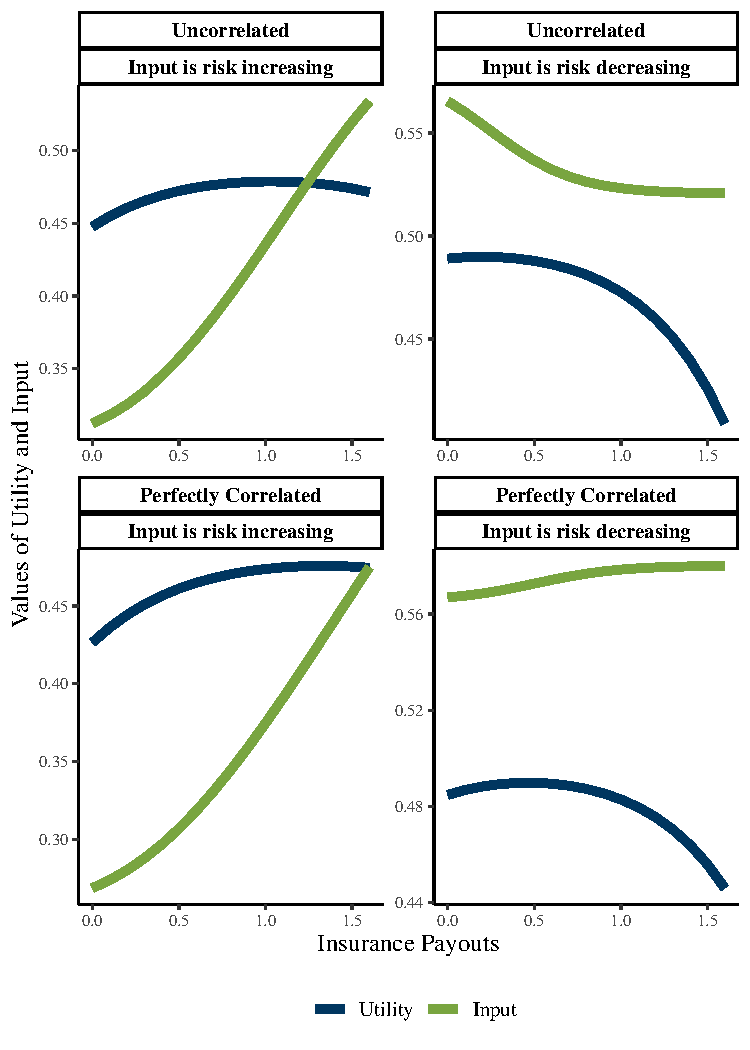
\includegraphics[keepaspectratio]{ibi-behavior_files/figure-pdf/fig-iter-1.pdf}}

}

\caption{\label{fig-iter}Improvements in utility (green lines) and
changes in optimal input use (blue lines) with index insurance. Shocks
are uncorrelated with high mean productivity (\(\alpha=0.75\)), high
risk aversion \(a=3\), and relatively more variable weather shocks than
biological (\(\sigma_{w}=0.4\) vs \(\sigma_{t}=0.1\))}

\end{figure}%

Optimal input use changes monotonically with index insurance depending
on the risk characteristics of the input (Figure~\ref{fig-iter}). The
direction of all input changes follows expected theory. The bottom right
panel shows the new instance where a risk decreasing monotonically
increases when the shocks are correlated following
Proposition~\ref{prp-corr}.

The concavity of utility, as demonstrated by the blue parabolas in all
panels of Figure~\ref{fig-iter}, implies there exists an optimal amount
of insurance for fishers to buy. The monotoncity of input use in all
cases suggests that the insurance level that maximizes utility will
preserve the sign of input changes. Therefore, an endogenous choice of
insurance will not affect the direction of input change, but it will
affect the magnitude.

For example, risk increasing inputs have higher levels of insurance
payouts that maximize utility. Allowing fishers to choose insurance
coverage ensures that the choice of insurance and input use changes are
welfare improving and will not bias input choices with over or under
investment of insurance. Simulations moving forward will allow fishers
to choose both inputs and insurance coverage.

Adding an endogenous \(\gamma\) to Equation~\ref{eq-maxsim} amends the
choice set in Equation~\ref{eq-maxsim2}. Furthermore, we run two groups
of simulations. One with the insurance contracted indemnified on
\(\omega\) as shown in Equation~\ref{eq-maxsim}, and another with the
index built on \(\theta\) to test all conditions of
Proposition~\ref{prp-ind} and Proposition~\ref{prp-corr}.

\begin{equation}\phantomsection\label{eq-maxsim2}{
\begin{aligned}
U&\equiv\max_{x,\gamma}\mathbb{E}[u]=\mathbb{E}[(1-\exp(-a(\pi(x,\hat\beta,\theta,\omega)+\mathbb{I}(\gamma))]\\
\mathbb{I}(\gamma)&=\begin{cases}-\rho\gamma & \text{if } \omega\ge \bar\omega\\
(1-\rho)\gamma & \text{if } \omega<\bar\omega
\end{cases}
\end{aligned}
}\end{equation}

Correlation between stock and extraction risk impact optimal choice of
input in line with Proposition~\ref{prp-ind} and
Proposition~\ref{prp-corr} when contracts use \(\omega\) as the index.
The clusters of bar graphs furthest to the left along the x-axis in each
panel are changes in input use when shocks are uncorrelated
(Figure~\ref{fig-corr}). Uncorrelated shocks have consistent signs of
input use in accordance to the underlying inputs risk effect function.
The bars in red indicate the input is risk decreasing, while the blue
bars are risk increasing. The stronger the risk effect, the more
pronounced the change in input use. All risk decreasing inputs had lower
input use when shocks are uncorrelated while all risk increasing inputs
saw higher use.

The productivity of inputs strongly influences the change in input use
particularly for risk decreasing inputs. When inputs are relatively less
productive (left panel, \(\alpha=0.25\)), fishers are more willing to
reduce the unproductive input in favor of the protection offered by
insurance. They lose less in production while gaining more variance
reduction by substituting with insurance. As productivity increases,
fishers would prefer to keep extracting at more efficient levels than
reduce input use. This tension is the primary driver towards higher risk
decreasing input use when the shocks become correlated.

Perfectly correlated shocks, shown by the far right cluster of bars in
each panel, show that risk increasing inputs will always see more use,
while risk decreasing inputs use could be lower or higher depending on
the relative productivity. The tradeoff between the risk reducing
capacity of the inputs and its marginal productivity drives this result.
Because the variables are perfectly correlated, insurance protects
against both stock and extraction risk. Insurance decreases the need to
reduce extraction risk through \(h(x)\), but increases the desire to
take on more stock risk to achieve greater harvests. Which of these
effects dominates depends on how productive is the input. Inputs with
low productivity do not provide as much benefit when taking on further
biological risk, so fishers will decrease their use if the input is risk
decreasing. Very productive inputs provide excellent marginal returns
and it becomes worthwhile to pursue additional harvest as insurance
protects the additional risk.

The more correlated the variables, the stronger the effect. The interior
cluster of bars in each panel show cases where the shocks are partially
correlated. Perfectly correlated indices imply zero basis risk and would
be considered ``perfect'' contracts. The behavioral implications of our
model suggest that this form of basis risk could lead to more
conservation degradation than imperfect uncorrelated contracts. However,
basis risk is a significant impediment to insurance uptake
(Binswanger-Mkhize 2012; Clarke 2016). Within our simulations, the
average improvement in utility for contracts with high basis risk was
1.5\%, and 7.8\% for ``perfect'' contracts implying that fisher demand
would be much higher for the perfect contract. If policymakers want to
promote well designed contracts, there must be other considerations to
curtail harvest expansion otherwise long run sustainability will be
impeded.

\begin{figure}

\centering{

\pandocbounded{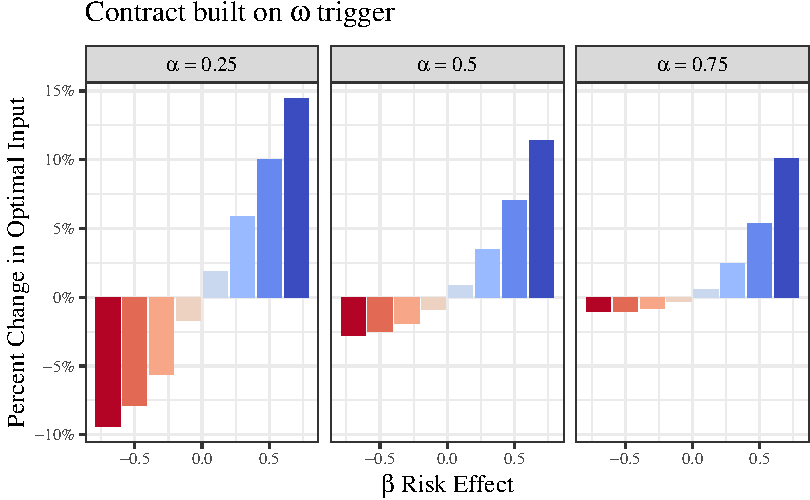
\includegraphics[keepaspectratio]{ibi-behavior_files/figure-pdf/fig-corr-1.pdf}}

}

\caption{\label{fig-corr}Percentage change in optimal input with an
index insurance contract using extraction risk, \(\omega\), as the
index. Risk increasing inputs (blue bars) always increase input use,
while risk decreasing inputs (red bars) have ambiguous effects depending
on the basis risk (correlation on the x-axis) and relative stock
productivity of the input (\(\alpha\) in the panels).}

\end{figure}%

Figure~\ref{fig-corr-theta} verifies the remaining properties of
Proposition~\ref{prp-ind} and Proposition~\ref{prp-corr}. Contracts
built on \(\theta\) as the index show more bias towards overfishing
because of the inherent risk increasing characteristics of \(f(x)\).
Uncorrelated shocks imply that insurance will only protect shocks on
\(\theta\). Production can expand as insurance protects the additional
risk of \(\theta f(x)\) regardless of the risk decreasing inputs. The
results become ambiguous when the shocks are correlated for the same
reasons as when contracts are built on \(\omega\). The overall
protection offered by insurance will allow whichever marginal effect
between \(h_x(x)\) and \(f_x(x)\) to dominate the direction of optimal
input use.

\begin{figure}

\centering{

\pandocbounded{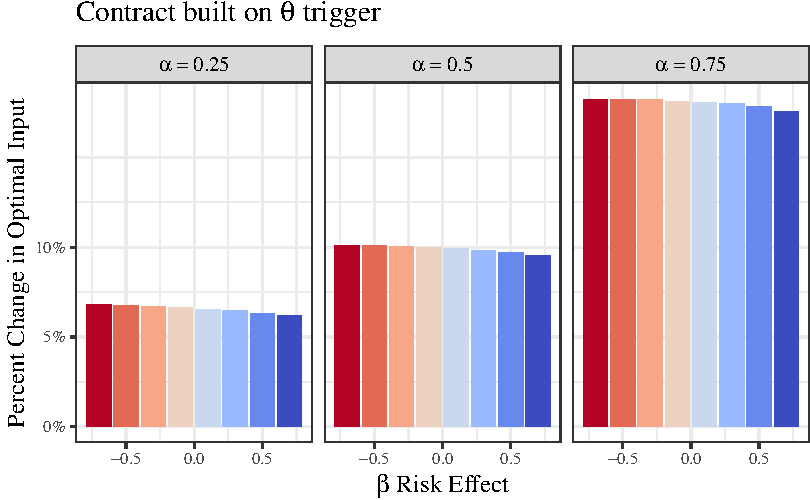
\includegraphics[keepaspectratio]{ibi-behavior_files/figure-pdf/fig-corr-theta-1.pdf}}

}

\caption{\label{fig-corr-theta}Percentage change in optimal input with
an index insurance contract indenmified on stock risk, \(\theta\).
Higher corrleations (x-axis) lead to amiguous results where \(\omega\)
risk decreasing inputs (red bars) could lead to decreases in input use.
Panels indicate the stock production elasticity. Risk increasing inputs
(blue bars) always lead to greater input use.}

\end{figure}%

Magnitude of input changes are sensitive to other parameters. More risk
averse fishers respond more aggressively to insurance and make
relatively more changes toward their input decisions (Panel A in
Figure~\ref{fig-sum}). Risk aversion implies more sensitivity towards
risk. The protection from insurance has greater marginal value for more
risk averse fishers. Greater marginal value of insurance means they can
invest less into risk reducing inputs than before, and have more
protection from greater shocks with risk increasing inputs.

Fisher input choice are much more responsive to insurance protection
from larger productivity risks (Panel B Figure~\ref{fig-sum}). Similar
to risk aversion, the greater the shocks the greater the marginal value
of insurance is to mitigate those shocks. In more volatile environments,
insurance provides significantly more income smoothing leading to
similar incentives as the higher risk aversion example.

Trigger levels do not appear to have differing impacts on input use.
Setting the trigger levels to more catastrophic coverage did not
encourage fishers to change their input use relative to the other
parameters. While necessary for applying Lemma~\ref{lem-mp} and
Lemma~\ref{lem-corr} in the proofs, the results of
Proposition~\ref{prp-ind} and Proposition~\ref{prp-corr} would appear to
hold if \(\bar\omega\ne0\) and \(\bar\theta\ne0\).

\begin{figure}

\centering{

\pandocbounded{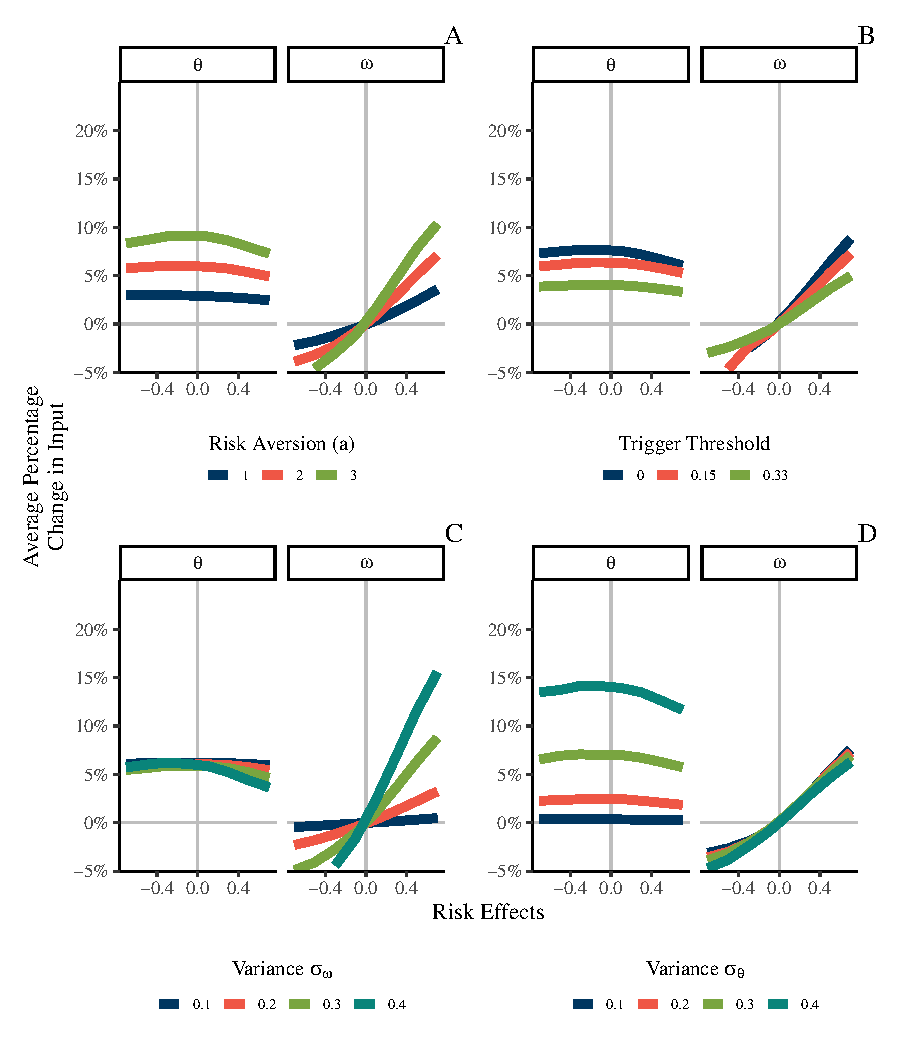
\includegraphics[keepaspectratio]{ibi-behavior_files/figure-pdf/fig-sum-1.pdf}}

}

\caption{\label{fig-sum}Risk Aversion (A), weather variance \(\omega\)
(B), and trigger (C) all influence the magnitude of change in harvest.
Mean production elasticity is set to 0.5. Average percent change in
input (y-axis) is summarized across all other parameter combinations for
each risk effect value of \(\beta\).}

\end{figure}%

In the next section we use parameters from Asche \emph{et al.} (2020) to
calculate the overall change in harvest with multiple inputs interacting
with index insurance.

\subsection{Application to Norwegian
Fisheries}\label{application-to-norwegian-fisheries}

Fishery extraction risk effects are rarely estimated, though appear
crucial to determining the magnitude of input change with index
insurance. The only known study to date that calculates risk effects is
that of Asche \emph{et al.} (2020). They used a non-linear estimator to
calculate the production and risk parameters of a Just-Pope function
across four different vessel types. We will use their coefficient
calculations to calibrate an estimate of the magnitude of input and
harvest change that index insurance would incentivize if offered to
important Norwegian fisheries.

Asche et al., (2020) aggregated by vessel type and not species, so there
is no reasonable estimate for biomass. They accounted for biomass using
fixed effects in their regression, but without additional information we
cannot parameterize the mean and variance of biomass. Therefore, our
simulations normalize mean biomass to 1 and we assume the stock shocks,
\(\theta\), have three degrees of correlation with \(\omega\),
\(\{0,0.5,1\}\). Norwegian fisheries are well managed so the stock
variance could be mitigated through quota systems or accurate stock
assessments. The simulation model uses three inputs: capital \(k\),
labor \(l\), and fuel \(f\) (Equation~\ref{eq-sim3}).

\begin{equation}\phantomsection\label{eq-sim3}{
\pi(k,l,f)=k^{\alpha_k}l^{\alpha_l}f^{\alpha_f}(\hat\beta+\theta)+\omega k^{\beta_k}l^{\beta_l}k^{\beta_f}-c_kk^2-c_ll^2-c_ff^2
}\end{equation}

Mean production, \(\alpha\), and risk, \(\beta\), elasticities control
the stock and extraction risk effects respectively. Each parameter is
indexed to a particular input through the subscript, e.g.~fuel mean
production elasticity is \(\alpha_f\). Fishers in the simulation choose
inputs and insurance coverage to maximize expected utility. We show
their choice based on a \(\omega\) contract
(Equation~\ref{eq-maxasche}), but also run a model specification with a
contract built on \(\theta\).

\begin{equation}\phantomsection\label{eq-maxasche}{
\begin{aligned}
U&\equiv\max_{\gamma,k,l,f}\mathbb{E}[u]=\mathbb{E}[u(k^{\alpha_k}l^{\alpha_l}f^{\alpha_f}(\hat\beta+\theta)+\omega k^{\beta_k}l^{\beta_l}k^{\beta_f}-c_kk^2-c_ll^2-c_ff^2+\mathbb{I}(\gamma)]\\
\mathbb{I}(\gamma)&=\begin{cases}-\rho\gamma & \text{if } \omega\ge \bar \omega\\
(1-\rho)\omega& \text{if } \omega<\bar \omega
\end{cases}
\end{aligned}
}\end{equation}

Table~\ref{tbl-asche} shows the production and risk elasticities of the
four vessel types used in the simulation. While not all elasticities
were found to be statistically different from zero, we used their raw
values because dropping only those variables that are significant in
both matching parameters would have kept only a few valid combinations.
All non-significant elasticities led to small changes, but their
interactions with other inputs could partially drive some of the
observed outcomes.

\begin{longtable}[]{@{}
  >{\raggedright\arraybackslash}p{(\linewidth - 12\tabcolsep) * \real{0.2609}}
  >{\raggedleft\arraybackslash}p{(\linewidth - 12\tabcolsep) * \real{0.1304}}
  >{\raggedleft\arraybackslash}p{(\linewidth - 12\tabcolsep) * \real{0.1304}}
  >{\raggedleft\arraybackslash}p{(\linewidth - 12\tabcolsep) * \real{0.1304}}
  >{\raggedleft\arraybackslash}p{(\linewidth - 12\tabcolsep) * \real{0.1159}}
  >{\raggedleft\arraybackslash}p{(\linewidth - 12\tabcolsep) * \real{0.1159}}
  >{\raggedleft\arraybackslash}p{(\linewidth - 12\tabcolsep) * \real{0.1159}}@{}}

\caption{\label{tbl-asche}Production and Risk elasticities of Norwegian
Fisheries from Asche et al., (2020)}

\tabularnewline

\toprule\noalign{}
\begin{minipage}[b]{\linewidth}\raggedright
\end{minipage} & \begin{minipage}[b]{\linewidth}\raggedleft
\(\alpha_k\)
\end{minipage} & \begin{minipage}[b]{\linewidth}\raggedleft
\(\alpha_l\)
\end{minipage} & \begin{minipage}[b]{\linewidth}\raggedleft
\(\alpha_f\)
\end{minipage} & \begin{minipage}[b]{\linewidth}\raggedleft
\(\beta_k\)
\end{minipage} & \begin{minipage}[b]{\linewidth}\raggedleft
\(\beta_l\)
\end{minipage} & \begin{minipage}[b]{\linewidth}\raggedleft
\(\beta_f\)
\end{minipage} \\
\midrule\noalign{}
\endhead
\bottomrule\noalign{}
\endlastfoot
Coastal Seiners & 0.294 & 0.421 & 0.457 & 0.184 & -0.432 & 0.119 \\
Coastal Groundfish & 0.463 & 0.421 & 0.355 & 0.965 & -0.080 & 0.113 \\
Purse Seiners & 0.941 & -0.108 & 0.605 & -0.454 & -0.231 & 0.160 \\
Groundfish Trawlers & 0.210 & 0.106 & 0.531 & -2.788 & -0.110 &
-0.024 \\

\end{longtable}

We use the same parameter space as the previous simulations to test the
sensitivity of fisher input choices with index insurance. We plot the
distribution of input change after insurance for all uncorrelated
combination of parameters in Figure~\ref{fig-asche-input} based on a
contract with \(\omega\) as the index. Figure~\ref{fig-asche-input} also
allow us to examine whether the conditions of
Proposition~\ref{prp-samre} hold with real world
combinations\footnote{Proposition~\ref{prp-samre} requires shocks to be
  uncorrelated otherwise ambiguity enters. Figure~\ref{fig-asche-all} in
  the appendix shows the same results with the entire correlation
  parameter set. The change in direction for each input becomes much
  more ambiguous as expected based on the results of
  Proposition~\ref{prp-corr}}. We report the highest density as an
indicator of the general direction of input change.

\begin{figure}

\centering{

\pandocbounded{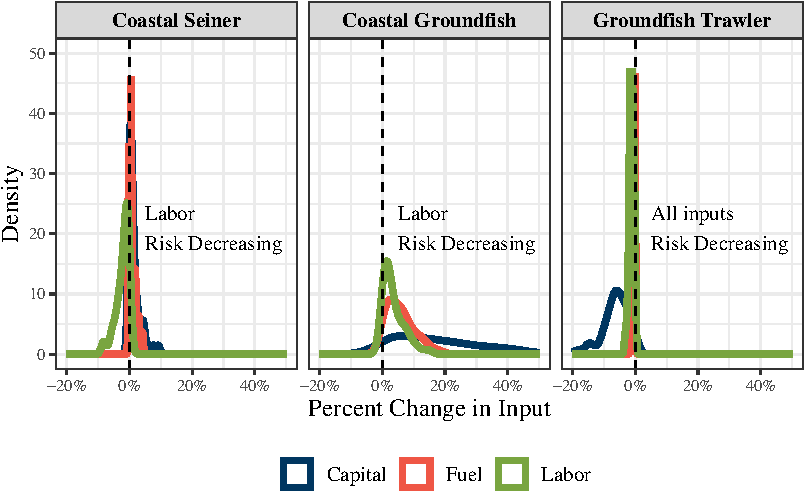
\includegraphics[keepaspectratio]{ibi-behavior_files/figure-pdf/fig-asche-input-1.pdf}}

}

\caption{\label{fig-asche-input}Density plots of the percent change in
input use for each vessel type in Norwegian fisheries. The dashed black
line represents no change in input use. Risk decreasing inputs are
labeled. Labor (green lines) is dropped for Purse Seiners because labor
was never used in simulations due to negative productivity elasticity.
Correlation between shocks is set to 0 in order to test the conditions
of Proposition 4.1}

\end{figure}%

Most changes in inputs tend to change in the direction expected of their
own individual risk effects. For example, fuel and capital are risk
increasing inputs for Coastal Seiners while labor is risk decreasing. In
the top left panel of Figure~\ref{fig-asche-input} the distribution of
the percent change in use for the risk increasing inputs (capital in
green and fuel in green) were always positive, and negative for the risk
decreasing input (labor in green). Despite the mix, each input follows
their respective input and demonstrates the conditions of
Proposition~\ref{prp-samre} can hold. The Groundfish Trawler fishery
also shows that the conditions of Proposition~\ref{prp-samre} hold. All
inputs are risk decreasing. The distribution of change in inputs in the
bottom right panel are negative.

The conditions of Proposition~\ref{prp-samre} do not hold in the case of
the Purse Seiner and Coastal Groundfish fisheries. The Purse Seiner
fishery never used labor due to the negative production elasticity.
Capital and fuel both saw positive and negative changes to their input
use despite capital being risk decreasing and fuel being risk
increasing. While there is no consistent pattern for what leads the
reversal in directions, it appears that when \(\theta\) variance is high
capital tends to dominate fuel risk so that the fisher choose less
capital and fuel. Higher \(\omega\) variance tends to lead fuel and
capital to both increase.

Labor in the Coastal Groundfish fishery is risk decreasing, yet always
saw an increase in the simulations. The risk parameter of labor is
relatively small compared to the risk increasing coefficients of capital
and fuel. The cross partial mix of the inputs may explain why fishers
add more labor. As insurance strongly incentivizes capital and fuel
increases, labor must also increase to further enhance those other
inputs.

Input changes lead to harvest changes. We examine the total change in
harvest for all parameters in Figure~\ref{fig-asche} for a contract
triggered on \(\omega\). Overall, insurance leads to relatively small
changes in harvest for all fisheries, but increases are stronger than
decreases. Coastal Groundfish see the largest and most consistent
increase in harvest. Median harvest increased by 12.5\% with a max
increase of 50\%. Coastal Groundfish have the most risk increasing
inputs out of the estimated fisheries and always saw increases in input
use (Figure~\ref{fig-asche-input}).

\begin{figure}

\centering{

\pandocbounded{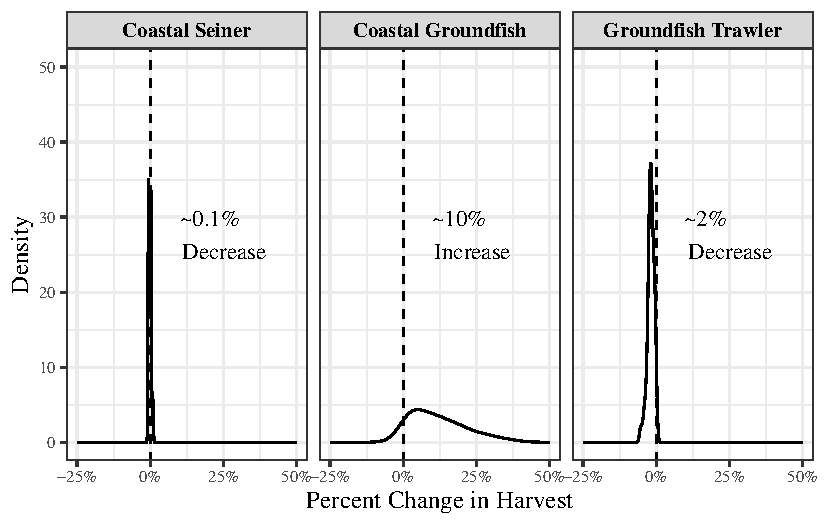
\includegraphics[keepaspectratio]{ibi-behavior_files/figure-pdf/fig-asche-1.pdf}}

}

\caption{\label{fig-asche}Density plots of the percent change in harvest
for each vessel type in Norwegian fisheries. The dashed line represents
no change in harvest. The text labels represent the median percent
change in harvest for each vessel type.}

\end{figure}%

Coastal Seiners had a relatively balanced spectrum of risk effects. The
input mix in this case led to both increases and decreases in input use,
which on net led to near zero changes in harvest. There is a slight skew
towards increased harvest, but drastically less than the Coastal
Groundfish fishery.

Deep water fleets generally saw reductions in harvest. Purse Seiners
tended to decrease harvest by 4\%. Groundfish trawlers consistently see
small decreases of 1.5\% in harvest (Figure~\ref{fig-asche}). All inputs
are risk decreasing with capital having the strongest risk effect out of
all inputs across all fisheries. However, it has a relatively low
marginal productivity. Insurance decreases trawler capital use by about
8\%, but the low productivity leads to only a 1.5\% decrease in overall
harvest.

Applying an insurance contract indemnified on \(\theta\) instead of
\(\omega\) shows similar results, but shifts the direction towards more
overfishing (Figure~\ref{fig-asche-theta}). The most prominent shifts
occur in the Groundfish Trawlers and Coastal Seiner fleets. In
Figure~\ref{fig-asche}, the percent change in harvest for Coastal
Seiners is indistinguishable from zero. With a \(\theta\) index
contract, there is now a pronounced shift towards overharvesting
(Figure~\ref{fig-asche-theta}).

Groundfish Trawlers have opposite results with a contract indemnified on
\(\theta\). Despite the risk decreasing dominance of capital, fishers
will choose to increase production as insurance drastically protects
against the added harvest risk. This result most clearly shows the
impact of different insurance contracts and the potential for
maladaptive behavior change. Without considering all the margins for
change, insurance protecting against biological risk will still
encourage overfishing without additional constraints.

\begin{figure}

\centering{

\pandocbounded{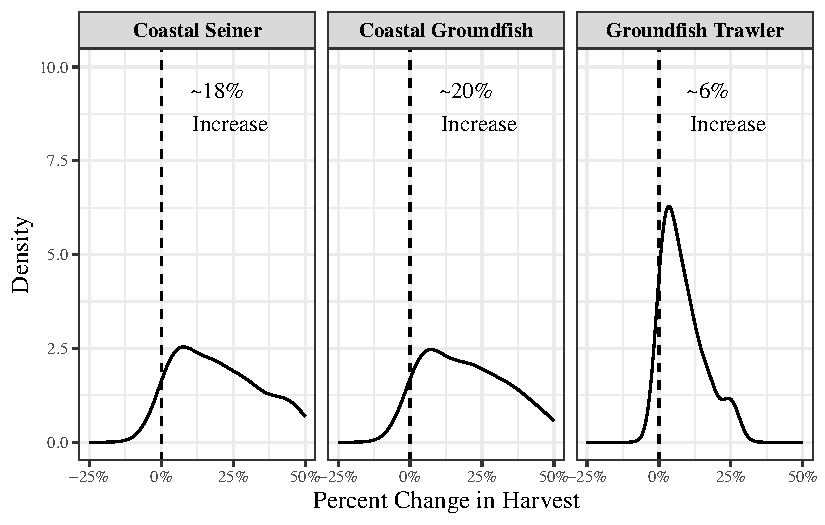
\includegraphics[keepaspectratio]{ibi-behavior_files/figure-pdf/fig-asche-theta-1.pdf}}

}

\caption{\label{fig-asche-theta}Density plots of the percent change in
harvest for each vessel type in Norwegian fisheries with insurance
contract indemnified on biological risk \(\theta\). The dashed line
represents no change in harvest. The text labels represent the median
percent change in harvest for each vessel type.}

\end{figure}%

\section{Discussion}\label{sec-disc}

This paper makes three distinct contributions. First, index insurance
will have behavioral impacts on fishers' input decisions, which in turn
will lead to changes in fishery sustainability. Second, the design of
index insurance contracts affects policyholder behavior contingent on
the mitigation strategies available to protect the underwritten risk.
Third, fishers face distinct sources of risk through the biology of fish
stocks and inherent harvesting variability that can be modeled with a
new stochastic production function.

The fundamental driver of fishers' behavior changes is whether the
marginal change in productivity is balanced by the marginal change in
risk. Fishers are more willing to increase production if insurance
negates the additional risk of expanded production. Since insurance
lowers risk, fishers need less self insurance through risk reducing
inputs and can reduce their overall input use. However, using less
inputs implies less catch and revenue creating a unique tension that
exists throughout the analysis. Across all simulations, decreased input
use was smaller than increased input use holding all other parameters
constant. Behavior change in fisheries will lean towards expanding
production creating a dilemma for conservation efforts.

Index insurance would improve welfare in Norwegian fisheries, but also
lead to changes in harvest that depends on the extraction risk effects
of fishing fleets. Coastal groundfish trawlers increased fishing
pressures by 12.5\% when offered insurance. Capital and fuel are risk
increasing inputs, and encourage the increased harvest. If an insurance
policy was applied to provide the income smoothing benefit of insurance,
the policymaker must take measures to mitigate the preserve incentive to
expand fishing production. Otherwise, the long term health of the stock
could be degraded and fishers would be worse off in the long run (Müller
\emph{et al.} 2017; John \emph{et al.} 2019; Bulte and Haagsma 2021).

Norwegian pelagic groundfish trawlers would have the opposite
considerations. When offered insurance they reduced their harvest by
1.5\%. Though small, it will lead to improved fishery sustainability.
The long term benefit of insurance would increase with improved stock
health. The decline in harvest was driven by a reduction in
overcapitalization, because capital was a significantly risk decreasing
input. Policymakers should attempt to identify fisheries with risk
decreasing inputs for insurance contracts to improve sustainability if
index insurance is to operate in isolation of other policies.

Ex-ante identification of input risk effects is challenging. Extraction
risk effects remain an elusive concept in fisheries, and need to
reconciled in order to articulate more accurate behavior changes of
fishery index insurance. Crop covers and pesticide provide clear
examples of risk decreasing inputs in agriculture, but what do risk
decreasing inputs look like in fisheries? Asche \emph{et al.} (2020)
provide empirical evidence of the existence of risk decreasing inputs,
but do not elaborate on why or how labor and capital directly decrease
risk. Labor is perhaps the more intuitive risk decreasing input.
Technical expertise of crew and captains can hedge against luck when
fishing (Alvarez \emph{et al.} 2006). Better trained crew can deploy
gear in a safe and timely manner, increasing the likelihood of effective
sets.

Fuel as a risk increasing input in fisheries makes intuitive sense as
well. Fuel is used to power vessels and is a direct cost of fishing.
Fishers explore productive fishing grounds for the best location. Every
hour at sea increases the harvest reward, but also the chances of
failure.

Capital is a more complex input, because it is shown to be both risk
increasing and decreasing. Capital in fisheries typically refer to
vessel tonnage, engine power, and gear technology. Greater capital
increases risk because it allows fishers to explore more fishing
grounds, use more efficient gear, and fish in more adverse weather
conditions. Alternatively, having larger vessels may be a risk reducing
input when common pool resources incentivize the race to fish, as the
sooner a fisher harvests from the stock, they assure their income at the
expense of other fishers. Adding risk aversion to standard models of
common pool fisheries suggests fishers should lower their capital use
compared to risk neutral allocations (Mesterton-Gibbons 1993; Tilman
\emph{et al.} 2018). Yet, overcapitalization and overfishing are more
often observed in the real world. Either fishers are never risk averse
or the risk effects of capital are not as simple as the standard model
suggests. When capital is allowed to be risk decreasing, optimal input
choices are much higher than risk neutral equilibrium suggesting fishers
are making rational, risk averse decisions even while overfishing.

Fishers exposure to multiple sources of risk further necessitates
insurance, but also makes it more challenging to design.
Proposition~\ref{prp-corr} shows the interaction between the stock and
extraction risk obscure the moral hazard of insurance. It is far more
likely that weather variables will have some degree of correlation. The
assumed volatility of more fish in the ocean leads the harvest function
to implicitly be risk increasing in our specification of stochastic
production. With this assumption, designing a contract around a stock
shock will bias the results towards more overfishing. In the Norwegian
fisheries, contracts built on stock risk increased median fish harvest
in all fisheries. However, the leading candidates for possible indices
in fisheries index insurance are currently weather variables most often
associated with biological stock risks (Watson \emph{et al.} 2023).
Designing contracts solely on these variables may lead to harvest
increases that run contrary to conservation goals.

However, most bioeconomic models simplify the complex effects of stock
dynamics into multiplicative or additive forms as modeled in this paper.
Instead, different forms of risk could be embedded into the biological
component of fishery models. Stock variance could be greater in
overfished stocks instead of healthier ones, reflecting more
vulnerability in weaker states (Sims \emph{et al.} 2018). Adapting
alternative, more biologically focused specifications of stock risk
could change the behavioral effects of insurance. Fishers may be more
willing to expose themselves to greater risk at more vulnerable stock
levels with insurance. Alternatively, insurance could help mitigate risk
and incentivize fishers to move toward healthier stocks with less
variance by alleviating income pressures to fish. Further analysis is
required to understand the full implications of stock risk effects in
fisheries.

The transfer between inputs and insurance reflects the substitution
between self-insurance and formal insurance (Quaas and Baumgärtner
2008). If index insurance is designed to reduce fishing capacity,
efforts must be made to ensure that it does not take away from the self
resiliency of fishers. Labor appears to be consistently risk reducing
and acts as a form of self insurance. If index insurance incentivizes
captains to hire less crew, the stock of fish may be preserved, but less
employment may reverberate throughout the community. Fishing is often a
primary employment opportunity in coastal communities. The resiliency of
the community would be compromised rather than enhanced with fewer jobs.
The same idea applies to capital. If fishers are over investing in
capital to hedge against some form of risk, policymakers need to be sure
the insurance is replacing maladaptive self insurance behavior.

The primary form of self insurance in fisheries is management. To this
point our analysis explicitly modeled scenarios without the existence of
management. We wanted to analyze the interaction of insurance on fisher
behavior in unconstrained settings first to derive a clearer incentive
structure. Most fisheries are managed in some form. The interaction
between management and insurance may be complementary or substitutes.
For example, well managed fisheries that have responsive harvest control
rules may not need insurance. The management system is already providing
the necessary risk protection. Insurance demand and uptake may be low in
these fisheries.

Insurance could instead complement management to provide the financial
relief that management cannot offer. Managers often focus on the
biological health of the fishery that can run at odds with fishers'
desires to enhance their income. Insurance can act as the financial
relief and allow managers to pursue more active strategies to protect
fish stocks without political resistance from lowered quotas.
Additionally, management can provide the constraints on insurance moral
hazard so the income smoothing benefits are passed to fishers, but not
the long term degradation. The interaction between insurance and
management requires further investigation especially with the the
numerous management strategies that exist in fisheries.

Design and access of insurance must also consider equity. The current US
federal disaster relief program is inequitable with bias towards large
industrial vessels (Jardine \emph{et al.} 2020). Creating another
program with equal inequity would be foolhardy. Current US farm
subsidies, including insurance premiums, are heavily skewed towards
large agribusinesses (White and Hoppe 2012). Dimensions of access,
procedural, representation, and distribution must all be built into the
design of new fishery index insurance programs (Fisher \emph{et al.}
2019). For example, small scale fishers may have income constraints that
prevent them from buying the initial contract. Micro-finance options
connected to insurance have been used in agriculture to alleviate this
burden with some success (Dougherty \emph{et al.} 2021). Additionally,
who receives the payouts needs thorough consideration. Payouts solely to
vessel owners may ignore support to valuable, yet vulnerable fishery
participants. Deckhands and crew are laid off during closures. The
broader community is also affected by lost income beyond fishers on the
water. Fish processors and harbors are also affected when fishing income
is lost. If index insurance payouts are going through the entire
fishery, the most vulnerable in the event of closures must be protected
as well. Contract stipulations could mandate that only cost expenses are
covered by payouts thereby including lost wages to the crew. Agriculture
contracts often are designed to directly cover expenses (He \emph{et
al.} 2020). Labor expenses could be included in the contract to ensure
that the crew is protected as well.

Our model only directly models behavior change through moral hazards.
Index insurance could be designed to incentivize other forms of
sustainable behavior change. We define three pathways insurance can
change behavior: Moral hazards, Quid Pro Quo, and Collective Action.
Moral hazards were proven in this paper to have ambiguous impacts
controlled by the risk characteristics of fishery inputs. The incentives
of moral hazards will always exist, therefore other measures could be
taken to either limit the downside behavioral effects of insurance or
stimulate other forms of sustainable behavior.

Quid Pro Quo expands contract design to explicitly build in conservation
measures. Fishers would be required to adopt sustainable practices in
order to qualify for insurance. Quid Pro Quo is already used in
agricultural insurance in the form of Good Farm Practices. Farmers must
submit management plans to US Risk Management Agency that clearly
outline their conservation practices in order to qualify for insurance.
Working closely with management agencies, insurance companies could
design contracts that require fishers to follow fishery specific
management practices. For example, fishers may be incentivized to use
more sustainable gear types, have an observer onboard, or reduce
bycatch. A stipulation in in the COAST program is for fishers to
register their vessels with the participating countries fisheries
department (Sainsbury \emph{et al.} (2019)). This step has brought
greater data clarity to small scale Caribbean fisheries.

Further research would need to uncover the full impact of Quid Pro Quo,
but an initial hypothesis would be the fishers will be willing to adopt
sustainable practices so long as the marginal gain in utility from the
insurance is greater or equal to the necessary sustainable changes.
Otherwise fishers will not want to buy the contracts and the insurance
has no binding stipulations to change the fishery.

Collective action ties insurance premiums to biological outcomes to
leverage the political economy of the fishery. Insures could reduce
premiums in fisheries that have robust management practices such as
adaptive harvest control rules, stock assessments, or marine protected
areas in the vicinity. Fishers could either pressure regulators to adopt
these actions or form industry groups to undertake the required actions.
Insurers would agree to this if triggers are connected to biological
health so that negative shocks are less frequent and thus payouts occur
less. Fishers gain from the reduced insurance premium and the increased
sustainability of harvest with rigorous management in place.

Ultimately, if index insurance is to be used in fisheries, it must be
designed with clear objectives and intentions. Index insurance can meet
objectives of income stability and risk reduction, but there has been an
implicit assumption by practitioners that index insurance will always
lead to improved sustainability. Without considering the behavior change
of fishers when adopting insurance, the outcomes may not be as expected.
New insights derived from this paper will help guide the efficient and
sustainable implementation of fisheries index insurance.

\newpage
\appendix
\renewcommand{\thefigure}{A\arabic{figure}}
\renewcommand{\thetable}{A\arabic{table}}
\setcounter{figure}{0}
\setcounter{table}{0}

\section{Appendix}\label{appendix}

\subsection{\texorpdfstring{Proof of
Lemma~\ref{lem-mp}}{Proof of Lemma~}}\label{proof-of-lem-mp}

\textbf{Lemma 3.1} \emph{Individual fisher expected marginal profit of a
specific input, \(x_m\), is greater in the good state than expected
marginal profit in the bad state when \(h_{x_m}(X)>0\). Expected
marginal profit is higher in the bad state when \(h_{x_m}(X)<0\). If
\(h_{x_m}(X)=0\), the marginal profits are equivalent in both states.}

\begin{proof}
By the first order conditions, there exist optimal values of any
individual input \(x_m\) that must be chosen before the realization of
the states of the world. Therefore \(h(X^*)\), \(f(X^*)\), and
\(c(X^*)\) are equal across states.

First we prove the case for contracts built on \(\omega\). The steps and
logic will follow nearly identically for \(\theta\).

Marginal utility in both states of the world is controlled by risk
effects and the sign of the random variables. Given \(\theta\) is
independent of \(\omega\), the expected value of
\(\mathbb{E}[\theta|\omega\lessgtr\bar\omega]=0\). The difference in
expected marginal profit across insurance states is defined as:

\begin{equation}\phantomsection\label{eq-comppi1}{
\begin{aligned}
\small
\frac{\partial \mathbb{E}[\pi|\omega<\bar\omega]}{\partial x^*_m}-\frac{\partial \mathbb{E}[\pi|\omega>\bar\omega]}{\partial x^*_m}=&\mathbb{E}[\omega h_{x_m^*}(X^*)|\omega<\bar\omega]+\cancel{f_{x_m^*}(X^*)\hat{B}}+\cancel{\mathbb{E}[\theta f_x(X^*)|\omega <\bar\omega]}-\cancel{c_{x^*_m}(X^*)} \\
&-\mathbb{E}[\omega h_{x_m^*}(X^*)|\omega>\bar\omega]+\cancel{f_{x_m^*}(X^*)\hat{B}}+\cancel{\mathbb{E}[\theta f_x(X^*)|\omega >\bar\omega]}-\cancel{c_{x^*_m}(X^*)}\\
=&\mathbb{E}[\omega h_{x_m^*}(X^*)|\omega<\bar\omega]-\mathbb{E}[\omega h_{x_m^*}(X^*)|\omega>\bar\omega]
\end{aligned}
}\end{equation}

If an input is risk decreasing then \(h_{x_m}(X)<0\). Then
Equation~\ref{eq-comppi1} is positive and marginal profit in the bad
state is greater than the marginal profit in the good state. Adding more
of a risk reducing input reduces the negative impact in the bad state
relative to the good state.

\[
\frac{\partial \mathbb{E}[\pi|\omega<\bar\omega]}{\partial x^*_m}-\frac{\partial \mathbb{E}[\pi|\omega>\bar\omega]}{\partial x^*_m}=\overbrace{\mathbb{E}[\omega h_{x_m^*}(X^*)|\omega<\bar\omega]-\mathbb{E}[\omega h_{x_m^*}(X^*)|\omega>\bar\omega]}^{+}
\]

Repeating the same steps for risk increasing inputs \(h_{x_m}(X)>0\)
shows that marginal profit in the bad state is less than marginal profit
in the good state.

\[
\frac{\partial \mathbb{E}[\pi|\omega<\bar\omega]}{\partial x^*_m}-\frac{\partial \mathbb{E}[\pi|\omega>\bar\omega]}{\partial x^*_m}=\overbrace{\mathbb{E}[\omega h_{x_m^*}(X^*)|\omega<\bar\omega]-\mathbb{E}[\omega h_{x_m^*}(X^*)|\omega>\bar\omega]}^{-}
\]

When the insurance contract is triggered on biological risk \(\theta\),
uncorrelated shocks will always lead to higher marginal profit in the
good state. Uncorrelated shocks lead
\(\mathbb{E}[\omega|\theta \lessgtr \bar \theta]=0\).

\begin{equation}\phantomsection\label{eq-compz}{
\begin{aligned}
\small
\frac{\partial \mathbb{E}[\pi|\theta<\bar\theta]}{\partial x^*_m}-\frac{\partial \mathbb{E}[\pi|\theta>\bar\theta]}{\partial x^*_m}=&\cancel{\mathbb{E}[\omega h_{x_m^*}(X^*)|\theta<\bar\theta]}+\cancel{f_{x_m^*}(X^*)\hat{B}}+\mathbb{E}[\theta f_x(X^*)|\theta <\bar\theta]-\cancel{c_{x^*_m}(X^*)} \\
&-\cancel{\mathbb{E}[\omega h_{x_m^*}(X^*)|\theta>\bar\theta]}-\cancel{f_{x_m^*}(X^*)\hat{B}}-\mathbb{E}[\theta f_x(X^*)|\theta >\bar\theta]+\cancel{c_{x^*_m}(X^*)}\\
=&\mathbb{E}[\theta f_x(X^*)|\theta <\bar\theta]-\mathbb{E}[\theta f_x(X^*)|\theta >\bar\theta]
\end{aligned}
}\end{equation}

The concavity of \(f(X)\) leads to \(f_x(X)>0\) always.
Equation~\ref{eq-compz} can then be signed to always be negative so that
marginal profit in the good state is always higher when insurance
contracts are triggered on \(\theta\).

\[
\frac{\partial \mathbb{E}[\pi|\theta<\bar\theta]}{\partial x^*_m}-\frac{\partial \mathbb{E}[\pi|\theta>\bar\theta]}{\partial x^*_m}=\overbrace{\mathbb{E}[\theta f_{x_m^*}(X^*)|\theta<\bar\theta]-\mathbb{E}[\theta f_{x_m^*}(X^*)|\theta>\bar\theta]}^{-}
\]
\end{proof}

\subsection{\texorpdfstring{Proof of
Lemma~\ref{lem-corr}}{Proof of Lemma~}}\label{proof-of-lem-corr}

\textbf{Lemma 3.2} \emph{When shocks are perfectly correlated, expected
marginal profit is always higher in the good state when an input,
\(x_m\), is risk increasing and ambiguous when \(x_m\) is risk
decreasing. This hold regardless of the chosen index.}

\emph{\(\frac{\mathbb{E}[\partial \pi|\omega<\bar \omega]}{\partial x_m}-\frac{\mathbb{E}[\partial \pi|\omega>\bar \omega]}{\partial x_m}<0\)
if \(h_{x_m}(X)>0\)}

\emph{And,
\(\frac{\mathbb{E}[\partial \pi|\omega<\bar \omega]}{\partial x_m}-\frac{\mathbb{E}[\partial \pi|\omega>\bar \omega]}{\partial x_m}\lessgtr 0\)
if \(h_{x_m}(X)<0\).}

\begin{proof}
Perfect correlation between two random variables centered at 0 imply
that whenever one variable is negative, so too is the other. Due to
this, we focus only on \(\omega\) as the index. The proof follows
identically if replaced by an index on \(\theta\).

\begin{equation}\phantomsection\label{eq-corrmp}{
\begin{aligned}
\frac{\partial \mathbb{E}[\pi|\omega<\bar\omega]}{\partial x}-\frac{\partial \mathbb{E}[\pi|\omega>\bar\omega]}{\partial x}=\cancel{f_{x}(x)}\hat{B}+\mathbb{E}[\theta f_x(x)|\omega<\bar\omega]+\mathbb{E}[\omega h_{x}(x)|\omega<\bar\omega]-\cancel c(x)\\
-\cancel{f_{x}(x)}\hat{B}+\mathbb{E}[\theta f_x(x)|\omega>\bar\omega]+\mathbb{E}[\omega h_{x}(x)|\omega>\bar\omega]-\cancel c(x)
\end{aligned}
}\end{equation}

When \(h_x(X)>0\), Equation~\ref{eq-corrmp} is always negative. Expected
marginal profit is always higher in the good trigger state when shocks
are perfectly correlated.

When \(h_x(X)<0\), Equation~\ref{eq-corrmp} is ambiguous. The sign of
each line depends on the relative effect between \(f_x(X)\) and
\(h_x(X)\). If the risk effects term dominates then
Equation~\ref{eq-corrmp} will be positive. Without further information
it is impossible to know which effect dominates.
\end{proof}

\subsection{\texorpdfstring{Proof of
Proposition~\ref{prp-samre}}{Proof of Proposition~}}\label{sec-samre}

\textbf{Proposition 4.1} \emph{In fisheries with two inputs, when
\(\theta\) and \(\omega\) are uncorrelated, index insurance will change
the optimal use of a specific input in accordance to an input's own risk
effect when the following sufficient condition is true:}

\emph{\(\frac{\partial U}{\partial x_a x_b}>0\) when both inputs share
the same risk effects, and
\(\frac{\partial U}{\partial x_a \partial x_b}<0\) when inputs have
opposite risk effects}

\emph{Otherwise, index insurance will have ambiguous effects on optimal
input choice.}

\begin{proof}
We use the same insurance design from Section~\ref{sec-common}. Fishers
now maximize expected utility by selecting two inputs. Contracts are
built on \(\omega\), but all steps follow for \(\theta\).

\begin{equation}\phantomsection\label{eq-max2}{
\begin{aligned}
U\equiv\max_{x_a,x_b}\mathbb{E}[U]=\int^{\infty}_{-\infty}&\left[ \int^{\bar \omega}_{-\infty}j_{\omega,\theta}(\omega,\theta)u(\pi(X,\hat{B},\theta,\omega)+(1-J(\bar \omega))\gamma)d\omega \right.\\
&\left.+\int^{\infty}_{\bar{\omega}}j_{\omega,\theta}(\omega,\theta) u(\pi(X,\hat{B},
\theta,\omega)-J(\bar \omega)\gamma)d\omega\right] d\theta
\end{aligned}
}\end{equation}

Taking the first order conditions yields:

\begin{equation}\phantomsection\label{eq-foc2}{
\begin{aligned}
\frac{\partial U}{\partial x_a}=&\int^{\infty}_{-\infty}\left[ \int^{\bar \omega}_{-\infty}j_{\omega,\theta}(\omega,\theta)u_{x_a}(\pi(X,\hat{B},\theta,\omega)+(1-J(\bar \omega))\gamma)\frac{\partial \pi}{\partial x_a}(X,\hat{B},\theta,\omega)d\omega\right.\\
&\left.+\int^{\infty}_{\bar{\omega}}j_{\omega,\theta}(\omega,\theta) u_{x_a}(\pi(X,\hat{B},\theta,\omega)-J(\bar \omega)\gamma)\frac{\partial \pi}{\partial x_a}(X,\hat{B},\theta,\omega)d\omega\right] d\theta\\
&=0\\
\frac{\partial U}{\partial x_b}=&\int^{\infty}_{-\infty}\left[ \int^{\bar \omega}_{-\infty}j_{\omega,\theta}(\omega,\theta)u_{x_b}(\pi(X,\hat{B},\theta,\omega)+(1-J(\bar \omega))\gamma)\frac{\partial \pi}{\partial x_b}(X,\hat{B},\theta,\omega)d\omega\right.\\
&\left.+\int^{\infty}_{\bar{\omega}}j_{\omega,\theta}(\omega,\theta) u_{x_b}(\pi(X,\hat{B},\theta,\omega)-J(\bar \omega)\gamma)\frac{\partial \pi}{\partial x_b}(X,\hat{B},\theta,\omega)d\omega\right] d\theta\\
&=0
\end{aligned}
}\end{equation}

Assuming the first order condition is satisfied, we can use the implicit
function theorem (IFT) to look at the impact of a change in the
exogenous insurance contract. Applying IFT yields a system of equations
that determine the impact of insurance on each optimal input:

\begin{equation}\phantomsection\label{eq-ivtsol}{
\begin{aligned}
&\frac{\partial x_a}{\partial \gamma}=\frac{-1}{Det}\left[\frac{\partial U}{\partial x_b \partial x_b}\frac{\partial U}{\partial x_a \partial \gamma}-\frac{\partial U}{\partial x_a \partial x_b}\frac{\partial U}{\partial x_b \partial \gamma}\right] \\
&\frac{\partial x_b}{\partial \gamma}=\frac{-1}{Det}\left[\frac{-\partial U}{\partial x_b \partial x_a}\frac{\partial U}{\partial x_a \partial \gamma}+\frac{\partial U}{\partial x_a \partial x_a}\frac{\partial U}{\partial x_b \partial \gamma}\right]
\end{aligned}
}\end{equation}

Because the DET will always be positive by the second-order condition,
we can focus on the interior of the brackets. If positive, then
insurance will lower use of that specific input and vice versa. The
partial derivatives in Equation~\ref{eq-ivtsol} are complex. Their
complete derivations are included in Section~\ref{sec-partial}.

Lemma~\ref{lem-mp} allows us to sign the partial equations
Equation~\ref{eq-kgam} and Equation~\ref{eq-lgam} for any risk effect on
either input. Concave utility by definition leads to \(u''<0\). For
simplicity, we will only focus on
\(\frac{\partial U}{\partial x_a\partial \gamma}\), but all applies
equally to \(\frac{\partial U}{\partial x_b\partial \gamma}\). Insurance
payouts equalize profits between different states. If insurance
completely covers all loss and \(x_a\) is risk increasing, then
\(\frac{\partial U}{\partial x_a\partial \gamma}\) is positive.

\begin{equation}\phantomsection\label{eq-kgamsol}{
\begin{aligned}
\frac{U}{\partial x_a \partial \gamma}=\int^{\infty}_{-\infty}&\overbrace{j_{\theta}(\theta)J(\bar\theta)(1-J(\bar\theta))u''(\theta,\cdot)}^{-}\\
&\left[ \int^{\bar\omega}_{-\infty}\underbrace{j_{\omega}(\omega)\frac{\partial \pi}{\partial x_a}d\omega
-\int^{\infty}_{\bar{\theta}}j_{\omega}(\omega)\frac{\partial \pi}{\partial x_a}d\omega}_{-}\right] d\theta\\
>0
\end{aligned}
}\end{equation}

Suppose both inputs are risk increasing so
\(\frac{\partial U}{\partial x_a\partial \gamma}\) and
\(\frac{\partial U}{\partial x_b\partial \gamma}\) are positive. The
only way for Equation~\ref{eq-ivtsol} to be unambiguously positive is
for \(\frac{\partial U}{\partial x_a\partial x_b}\) and
\(\frac{\partial U}{\partial x_a\partial x_b}\) to be positive.

\[
\begin{aligned}
&\frac{\partial x_a}{\partial \gamma}=\overbrace{\frac{-1}{Det}}^{-}\left[\overbrace{\overbrace{\frac{\partial U}{\partial x_b \partial x_b}}^{-}\overbrace{\frac{\partial U}{\partial x_a \partial \gamma}}^{+}\overbrace{-\frac{\partial U}{\partial x_a \partial x_b}}^{-}\overbrace{\frac{\partial U}{\partial x_b \partial \gamma}}^{+}}^{-}\right] >0\\
&\frac{\partial x_b}{\partial \gamma}=\overbrace{\frac{-1}{Det}}^{-}\left[\overbrace{\overbrace{\frac{-\partial U}{\partial x_b \partial x_a}}^{-}\overbrace{\frac{\partial U}{\partial x_a \partial \gamma}}^{+}+\overbrace{\frac{\partial U}{\partial x_a \partial x_a}}^{-}\overbrace{\frac{\partial U}{\partial x_b \partial \gamma}}^{+}}^{-}\right]>0
\end{aligned}
\]

Both risk increasing inputs will be raised with index insurance.
Repeating the same steps above with risk decreasing inputs shows both
inputs unambiguously decrease with index insurance.

Now suppose inputs have mixed risk effects. For simplicity, \(x_a\) will
be risk increasing and \(x_b\) will be risk decreasing. The results will
hold for the opposite case. By Lemma~\ref{lem-mp},
\(\frac{\partial U}{\partial x_a\partial \gamma}\) is positive, while
\(\frac{\partial U}{\partial x_b\partial \gamma}\) is negative.
Equation~\ref{eq-ivtsol} will be unambiguously positive if
\(\frac{\partial U}{\partial x_a\partial x_b}\) and
\(\frac{\partial U}{\partial x_b\partial x_a}\) are negative.

\[
\begin{aligned}
&\frac{\partial x_a}{\partial \gamma}=\overbrace{\frac{-1}{Det}}^{-}\left[\overbrace{\overbrace{\frac{\partial U}{\partial x_b\partial x_b}}^{-}\overbrace{\frac{\partial U}{\partial x_a \partial \gamma}}^{+}\overbrace{-\frac{\partial U}{\partial x_a \partial x_b}}^{+}\overbrace{\frac{\partial U}{\partial x_b\partial \gamma}}^{-}}^{-}\right] >0\\
&\frac{\partial x_b}{\partial \gamma}=\overbrace{\frac{-1}{Det}}^{-}\left[\overbrace{\overbrace{\frac{-\partial U}{\partial x_b\partial x_a}}^{+}\overbrace{\frac{\partial U}{\partial x_a \partial \gamma}}^{+}+\overbrace{\frac{\partial U}{\partial x_a \partial x_a}}^{-}\overbrace{\frac{\partial U}{\partial x_b\partial \gamma}}^{-}}^{+}\right]<0
\end{aligned}
\]

The risk increasing input will be raised with index insurance, while the
risk decreasing input will be lowered.

If these conditions do not hold, then it is impossible to determine
which additive element outweighs the other, and the insurance effects on
optimal input use will be ambiguous regardless of the underlying risk
effects of an input.
\end{proof}

\subsection{Partial derivatives}\label{sec-partial}

Partial derivatives used to sign Equation~\ref{eq-ivtsol} are shown
below. For brevity, \(\pi(X,\hat B,\omega,\theta)\) is reduced to
\(\pi\).

\begin{equation}\phantomsection\label{eq-kk}{
\begin{aligned}
\frac{\partial U}{\partial x_a \partial x_a}=\int^\infty_{-\infty}&\left[ \int^{\bar \omega}_{-\infty}j_{\omega,\theta}(\omega,\theta)[u''(\pi+(1-J(\bar \omega))\gamma)\frac{\partial\pi}{\partial x_a}+u'(\pi+(1-J(\bar \omega))\gamma)\frac{\partial \pi}{\partial x_a x_a}]d\omega \right. \\
&\left. +\int^\infty_{\bar \omega}j_{\omega,\theta}(\omega,\theta)[u''(\pi-J(\bar \omega)\gamma)\frac{\partial\pi}{\partial x_a}+u'(\pi-J(\bar \omega)\gamma)\frac{\partial \pi}{\partial x_a x_a}]d\omega\right]d\theta
\end{aligned}
}\end{equation}

\begin{equation}\phantomsection\label{eq-ll}{
\begin{aligned}
\frac{\partial U}{\partial x_b \partial x_b}=\int^\infty_{-\infty}&\left[ \int^{\bar \omega}_{-\infty}j_{\omega,\theta}(\omega,\theta)[u''(\pi+(1-J(\bar \omega))\gamma)\frac{\partial\pi}{\partial x_b}+u'(\pi+(1-J(\bar \omega))\gamma)\frac{\partial \pi}{\partial x_b x_b}]d\omega \right. \\
&\left.\int^\infty_{\bar \omega}j_{\omega,\theta}(\omega,\theta)[u''(\pi-J(\bar \omega)\gamma)\frac{\partial\pi}{\partial x_b}+u'(\pi-J(\bar \omega)\gamma)\frac{\partial \pi}{\partial x_b x_b}]d\omega\right]d\theta
\end{aligned}
}\end{equation}

\begin{equation}\phantomsection\label{eq-crossl}{
\begin{aligned}
\frac{\partial U}{\partial x_a \partial x_b}=\int^\infty_{-\infty}&\left[ \int^{\bar \omega}_{-\infty}j_{\omega,\theta}(\omega,\theta)[u''(\pi+(1-J(\bar \omega))\gamma)\frac{\partial\pi}{\partial x_a}\frac{\partial \pi}{\partial x_b}+u'(\pi+(1-J(\bar \omega))\gamma)\frac{\partial \pi}{\partial x_a x_b}]d\omega \right. \\
& \left.\int^\infty_{\bar \omega}j_{\omega,\theta}(\omega,\theta)[u''(\pi-J(\bar \omega)\gamma)\frac{\partial\pi}{\partial x_a}\frac{\partial \pi}{\partial x_b}+u'(\pi-J(\bar \omega)\gamma)\frac{\partial \pi}{\partial x_a x_b}]d\omega\right]d\theta
\end{aligned}
}\end{equation}

\begin{equation}\phantomsection\label{eq-crossk}{
\begin{aligned}
\frac{\partial U}{\partial x_b \partial x_a}=\int^\infty_{-\infty}&\left[ \int^{\bar \omega}_{-\infty}j_{\omega,\theta}(\omega,\theta)[u''(\pi+(1-J(\bar \omega))\gamma)\frac{\partial\pi}{\partial x_a}\frac{\partial \pi}{\partial x_b}+u'(\pi+(1-J(\bar \omega))\gamma)\frac{\partial \pi}{\partial x_b x_a}]d\omega \right. \\
& \left.\int^\infty_{\bar \omega}j_{\omega,\theta}(\omega,\theta)[u''(\pi-J(\bar \omega)\gamma)\frac{\partial\pi}{\partial x_a}\frac{\partial \pi}{\partial x_b}+u'(\pi-J(\bar \omega)\gamma)\frac{\partial \pi}{\partial x_b x_a}]d\omega\right]d\theta
\end{aligned}
}\end{equation}

\begin{equation}\phantomsection\label{eq-kgam}{
\begin{aligned}
\frac{\partial U}{\partial x_a \partial \gamma}=\int^\infty_{-\infty}&\left[ \int^{\bar \omega}_{-\infty}j_{\omega,\theta}(\omega,\theta)u''(\pi+(1-J(\bar \omega))\gamma)\frac{\partial\pi}{\partial x_a}(1-J(\bar \omega)d\omega \right. \\
& \left.\int^\infty_{\bar \omega}j_{\omega,\theta}(\omega,\theta)u''(\pi-J(\bar \omega)\gamma)\frac{\partial\pi}{\partial x_a}(-J(\bar \omega))d\omega\right]d\theta
\end{aligned}
}\end{equation}

\begin{equation}\phantomsection\label{eq-lgam}{
\begin{aligned}
\frac{\partial U}{\partial x_b \partial \gamma}=\int^\infty_{-\infty}&\left[ \int^{\bar \omega}_{-\infty}j_{\omega,\theta}(\omega,\theta)u''(\pi+(1-J(\bar \omega))\gamma)\frac{\partial\pi}{\partial x_b}(1-J(\bar \omega)d\omega \right. \\
&\left.\int^\infty_{\bar \omega}j_{\omega,\theta}(\omega,\theta)u''(\pi-J(\bar \omega)\gamma)\frac{\partial\pi}{\partial x_b}(-J(\bar \omega))d\omega\right]d\theta
\end{aligned}
}\end{equation}

\subsection{Figures}\label{figures}

\begin{figure}

\centering{

\pandocbounded{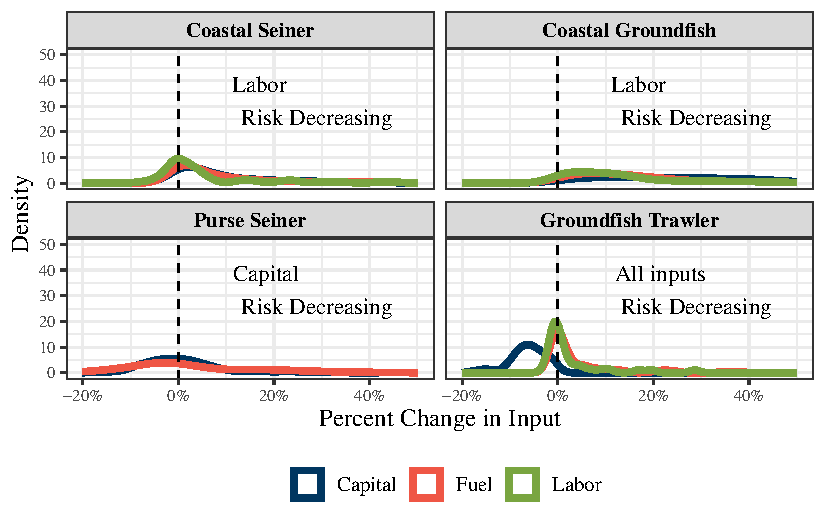
\includegraphics[keepaspectratio]{ibi-behavior_files/figure-pdf/fig-asche-all-1.pdf}}

}

\caption{\label{fig-asche-all}Density plots of the percent change in
input use for each vessel type in Norwegian fisheries. The dashed black
line represents no change in input use. Risk decreasing inputs are
labeled. Labor (green lines) is dropped for Purse Seiners because labor
was never used in simulations due to negative productivity elasticity.
Entire parameter space with correlations equal to 0, 0.5, and 1 used.}

\end{figure}%

\section*{References}\label{references}
\addcontentsline{toc}{section}{References}

\phantomsection\label{refs}
\begin{CSLReferences}{1}{0}
\bibitem[\citeproctext]{ref-Alvarez2006}
Alvarez, A., Schmidt, P., Alvarez, A. and Schmidt, P. (2006)
\href{https://doi.org/10.1007/s11123-006-0002-x}{Is skill more important
than luck in explaining fish catches?} \emph{J Prod Anal} \textbf{26},
15--25.

\bibitem[\citeproctext]{ref-Asche2020}
Asche, F., Cojocaru, A.L., Pincinato, R.B.M. and Roll, K.H. (2020)
\href{https://doi.org/10.1007/s10640-019-00391-2}{Production risk in the
norwegian fisheries}. \emph{Environmental and Resource Economics}
\textbf{75}, 137--149.

\bibitem[\citeproctext]{ref-Babcock1996}
Babcock, B.A. and Hennessy, D.A. (1996)
\href{https://doi.org/10.2307/1243713}{Input demand under yield and
revenue insurance}. \emph{American Journal of Agricultural Economics}
\textbf{78}, 416--427.

\bibitem[\citeproctext]{ref-Barbeaux2020}
Barbeaux, S.J., Holsman, K. and Zador, S. (2020)
\href{https://doi.org/10.3389/fmars.2020.00703}{Marine heatwave stress
test of ecosystem-based fisheries management in the gulf of alaska
pacific cod fishery}. \emph{Frontiers in Marine Science} \textbf{7},
1--21.

\bibitem[\citeproctext]{ref-binswanger2012}
Binswanger-Mkhize, H.P. (2012)
\href{https://doi.org/10.1080/00220388.2011.625411}{Is there too much
hype about index-based agricultural insurance?} \emph{Journal of
Development Studies} \textbf{48}, 187--200.

\bibitem[\citeproctext]{ref-Bulte2021}
Bulte, E. and Haagsma, R. (2021)
\href{https://doi.org/10.1007/s10640-021-00545-1}{The welfare effects of
index-based livestock insurance: Livestock herding on communal lands}.
\emph{Environmental and Resource Economics} \textbf{78}, 587--613.

\bibitem[\citeproctext]{ref-Cai2016}
Cai, J. (2016) \href{https://doi.org/10.1257/pol.20130371}{The impact of
insurance provision on household production and financial decisions}.
\emph{American Economic Journal: Economic Policy} \textbf{8}, 44--88.

\bibitem[\citeproctext]{ref-Carter2017}
Carter, M., Janvry, A.D., Sadoulet, E. and Sarris, A. (2017)
\href{https://doi.org/10.1146/annurev-resource-100516-053352}{Index
insurance for developing country agriculture: A reassessment}.
\emph{Annual Review of Resource Economics} \textbf{9}, 421--438.

\bibitem[\citeproctext]{ref-Cavole2016}
Cavole, L.M., Demko, A.M., Diner, R.E., et al. (2016)
\href{https://doi.org/10.5670/oceanog.2016.32}{Biological impacts of the
2013--2015 warm-water anomaly in the northeast pacific: Winners, losers,
and the future}. \emph{Oceanography} \textbf{29}, 273--285.

\bibitem[\citeproctext]{ref-Cheung2021}
Cheung, W.W.L., Frölicher, T.L., Lam, V.W.Y., et al. (2021)
\href{https://www.science.org}{Marine high temperature extremes amplify
the impacts of climate change on fish and fisheries}. \emph{Sci. Adv}
\textbf{7}.

\bibitem[\citeproctext]{ref-Claassen2017}
Claassen, R., Langpap, C. and Wu, J. (2017)
\href{https://doi.org/10.1093/AJAE/AAW075}{Impacts of federal crop
insurance on land use and environmental quality}. \emph{American Journal
of Agricultural Economics} \textbf{99}, 592--613.

\bibitem[\citeproctext]{ref-Clarke2016}
Clarke, D.J. (2016) \href{https://doi.org/10.1257/mic.20140103}{A theory
of rational demand for index insurance}. \emph{Journal: Microeconomics}
\textbf{8}, 283--306.

\bibitem[\citeproctext]{ref-Collier2009}
Collier, B., Skees, J. and Barnett, B. (2009)
\href{https://doi.org/10.1057/gpp.2009.11}{Weather index insurance and
climate change: Opportunities and challenges in lower income countries}.
\emph{Geneva Papers on Risk and Insurance: Issues and Practice}
\textbf{34}, 401--424.

\bibitem[\citeproctext]{ref-Deryugina2017}
Deryugina, T. and Konar, M. (2017)
\href{https://doi.org/10.1016/j.advwatres.2017.03.013}{Impacts of crop
insurance on water withdrawals for irrigation}. \emph{Advances in Water
Resources} \textbf{110}, 437--444.

\bibitem[\citeproctext]{ref-Dougherty2021}
Dougherty, J.P., Gallenstein, R.A. and Mishra, K. (2021)
\href{https://doi.org/10.1093/jafeco/ejab003}{Impact of index insurance
on moral hazard in the agricultural credit market: Theory and evidence
from ghana}. \emph{Journal of African Economies} \textbf{00}, 1--31.

\bibitem[\citeproctext]{ref-Eggert2004}
Eggert, H. and Tveteras, R. (2004) Stochastic production and
heterogeneous risk preferences: Commercial fishers' gear choices.
\emph{American Journal of Agricultural Economics} \textbf{86}, 199--212.

\bibitem[\citeproctext]{ref-Elabed2016}
Elabed, G. and Carter, M. (2018) Ex-ante impacts of agricultural
insurance: Evidence from a field experiment in mali.

\bibitem[\citeproctext]{ref-fao2020}
FAO (2020) \href{https://doi.org/10.4060/ca9229en}{The state of world
fisheries and aquaculture 2020. Sustinability in action}. \emph{INFORM}
\textbf{32}.

\bibitem[\citeproctext]{ref-fao2022}
FAO (2022) World review of capture fisheries and aquaculture insurance
2022.

\bibitem[\citeproctext]{ref-Fisher2019}
Fisher, E., Hellin, J., Greatrex, H. and Jensen, N. (2019)
\href{https://doi.org/10.1111/dpr.12387}{Index insurance and climate
risk management: Addressing social equity}. \emph{Development Policy
Review} \textbf{37}, 581--602.

\bibitem[\citeproctext]{ref-Goodwin2004}
Goodwin, B.K., Vandeveer, M.L. and Deal, J.L. (2004) An empirical
analysis of acreage effects of participation in the federal crop
insurance program. \emph{American Journal of Agricultural Economics}
\textbf{86}, 1058--1077.

\bibitem[\citeproctext]{ref-Grassini2011}
Grassini, P., Thorburn, J., Burr, C. and Cassman, K.G. (2011)
\href{https://doi.org/10.1016/j.fcr.2010.09.012}{High-yield irrigated
maize in the western u.s. Corn belt: I. On-farm yield, yield potential,
and impact of agronomic practices}. \emph{Field Crops Research}
\textbf{120}, 142--150.

\bibitem[\citeproctext]{ref-He2020}
He, J., Zheng, X., Rejesus, R. and Yorobe, J. (2020)
\href{https://doi.org/10.1111/AGEC.12558}{Input use under
cost-of-production crop insurance: Theory and evidence}.
\emph{Agricultural Economics (United Kingdom)} \textbf{51}, 343--357.

\bibitem[\citeproctext]{ref-Heck2021}
Heck, N., Beck, M.W. and Reguero, B. (2021)
\href{https://doi.org/10.1016/j.marpol.2021.104698}{Storm risk and
marine fisheries: A global assessment}. \emph{Marine Policy}
\textbf{132}, 104698.

\bibitem[\citeproctext]{ref-Herrmann2004}
Herrmann, M., Greenberg, J., Hamel, C. and Geier, H. (2004)
\href{https://doi.org/10.1577/M02-086.1}{Extending federal crop
insurance programs to commercial fisheries: The case of bristol bay,
alaska, sockeye salmon}. \emph{North American Journal of Fisheries
Management} \textbf{24}, 352--366.

\bibitem[\citeproctext]{ref-Holland2008}
Holland, D.S. (2008)
\href{https://doi.org/10.1086/mre.23.3.42629621}{Are fishermen rational?
A fishing expedition}. \emph{Marine Resource Economics} \textbf{23},
325--344.

\bibitem[\citeproctext]{ref-horowitz1993}
Horowitz, J. and Lichtenberg, E. (1993) Insurance, moral hazard, and
chemical use in agriculture. \emph{American Journal of Agricultral
Economics} \textbf{75}, 926--935.

\bibitem[\citeproctext]{ref-Jardine2020}
Jardine, S.L., Fisher, M.C., Moore, S.K. and Samhouri, J.F. (2020)
\href{https://doi.org/10.1016/j.ecolecon.2020.106691}{Inequality in the
economic impacts from climate shocks in fisheries: The case of harmful
algal blooms}. \emph{Ecological Economics} \textbf{176}.

\bibitem[\citeproctext]{ref-John2019}
John, F., Toth, R., Frank, K., Groeneveld, J. and Müller, B. (2019)
\href{https://doi.org/10.1016/J.ECOLECON.2018.11.021}{Ecological
vulnerability through insurance? Potential unintended consequences of
livestock drought insurance}. \emph{Ecological Economics} \textbf{157},
357--368.

\bibitem[\citeproctext]{ref-Just1978}
Just, R.E. and Pope, R.D. (1978)
\href{https://doi.org/10.1016/0304-4076(78)90006-4}{Stochastic
specification of production functions and economic implications}.
\emph{Journal of Econometrics} \textbf{7}, 67--86.

\bibitem[\citeproctext]{ref-Kasperski2013}
Kasperski, S. and Holland, D.S. (2013)
\href{https://doi.org/10.1073/pnas.1212278110}{Income diversification
and risk for fishermen}. \emph{Proceedings of the National Academy of
Sciences of the United States of America} \textbf{110}, 2076--2081.

\bibitem[\citeproctext]{ref-Kirkley1998}
Kirkley, J. and Strand, I.E. (1998) Characterizing managerial skill and
technical efficiency in a fishery. \emph{Journal of Productivity
Analysis} \textbf{9}, 145--160.

\bibitem[\citeproctext]{ref-Kompas2004}
Kompas, T., Che, T.N. and Grafton, R.Q. (2004)
\href{https://doi.org/10.1080/0003684042000218561}{Technical efficiency
effects of input controls: Evidence from australia's banana prawn
fishery}. \emph{Applied Economics} \textbf{36}, 1631--1641.

\bibitem[\citeproctext]{ref-Lehodey2006}
Lehodey, P., Alheit, J., Barange, M., et al. (2006) Climate variability,
fish, and fisheries.

\bibitem[\citeproctext]{ref-Lichtenberg2022}
Lichtenberg, E. and Iglesias, E. (2022)
\href{https://doi.org/10.1016/j.jdeveco.2022.102883}{Index insurance and
basis risk: A reconsideration}. \emph{Journal of Development Economics}
\textbf{158}.

\bibitem[\citeproctext]{ref-Mahul2001}
Mahul, O. (2001) \href{https://doi.org/10.1111/0002-9092.00180}{Optimal
insurance against climatic experience}. \emph{American Journal of
Agricultural Economics} \textbf{83}, 593--604.

\bibitem[\citeproctext]{ref-Maltby2023}
Maltby, K.M., Acosta, L., Townhill, B., Touza, J., White, P. and Mangi,
S.C. (2023) \href{https://doi.org/10.1093/icesjms/fsac003}{Exploring
fishers' perceptions of index insurance and coral reef health in the
context of climate-driven changes in extreme events}. \emph{ICES Journal
of Marine Science} \textbf{80}, 2210--2221.

\bibitem[\citeproctext]{ref-Merino2022}
Merino, G., Urtizberea, A., Fu, D., et al. (2022)
\href{https://doi.org/10.1016/j.fishres.2022.106478}{Investigating
trends in process error as a diagnostic for integrated fisheries stock
assessments}. \emph{Fisheries Research} \textbf{256}.

\bibitem[\citeproctext]{ref-gibbons1993}
Mesterton-Gibbons, M. (1993)
\href{https://doi.org/10.1111/j.1939-7445.1993.tb00143.x}{Game-theoretic
resource modeling}. \emph{Natural Resource Modeling} \textbf{7},
93--147.

\bibitem[\citeproctext]{ref-Mishra2005}
Mishra, A.K., Nimon, R.W. and El-Osta, H.S. (2005)
\href{https://doi.org/10.1016/j.jenvman.2004.08.003}{Is moral hazard
good for the environment? Revenue insurance and chemical input use}.
\emph{Journal of Environmental Management} \textbf{74}, 11--20.

\bibitem[\citeproctext]{ref-muller2017}
Müller, B., Johnson, L. and Kreuer, D. (2017)
\href{https://doi.org/10.1016/j.gloenvcha.2017.06.010}{Maladaptive
outcomes of climate insurance in agriculture}. \emph{Global
Environmental Change} \textbf{46}, 23--33.

\bibitem[\citeproctext]{ref-muller2011}
Müller, B., Quaas, M.F., Frank, K. and Baumgärtner, S. (2011)
\href{https://doi.org/10.1016/j.ecolecon.2011.06.011}{Pitfalls and
potential of institutional change: Rain-index insurance and the
sustainability of rangeland management}. \emph{Ecological Economics}
\textbf{70}, 2137--2144.

\bibitem[\citeproctext]{ref-Mumford2009}
Mumford, J.D., Leach, A.W., Levontin, P. and Kell, L.T. (2009)
\href{https://doi.org/10.1093/icesjms/fsp100}{Insurance mechanisms to
mediate economic risks in marine fisheries}. \emph{ICES Journal of
Marine Science} \textbf{66}, 950--959.

\bibitem[\citeproctext]{ref-Murkowski2022}
Murkowski, L. (2022) Working waterfronts framework: A plan to grow and
support alaska's coastal and river communities.

\bibitem[\citeproctext]{ref-Oken2021}
Oken, K.L., Holland, D.S. and Punt, A.E. (2021)
\href{https://doi.org/10.1002/eap.2307}{The effects of population
synchrony, life history, and access constraints on benefits from fishing
portfolios}. \emph{Ecological Applications} \textbf{0}, 1--16.

\bibitem[\citeproctext]{ref-Outreville2014}
Outreville, J.F. (2014) Risk aversion, risk behavior, and demand for
insurance: A survey. \emph{Source: Journal of Insurance Issues}
\textbf{37}, 158--186.

\bibitem[\citeproctext]{ref-Pandori2019}
Pandori, L.L.M. and Sorte, C.J.B. (2019)
\href{https://doi.org/10.1111/oik.05886}{The weakest link: Sensitivity
to climate extremes across life stages of marine invertebrates}.
\emph{Oikos} \textbf{128}, 621--629.

\bibitem[\citeproctext]{ref-Pfeiffer2020}
Pfeiffer, L. (2020) \href{https://doi.org/10.1093/icesjms/fsaa145}{How
storms affect fishers' decisions about going to sea}. \emph{ICES Journal
of Marine Science} \textbf{77}, 2753--2762.

\bibitem[\citeproctext]{ref-Pfeiffer2022}
Pfeiffer, L., Petesch, T. and Vasan, T. (2022)
\href{https://doi.org/10.1086/716856}{A safer catch? The role of
fisheries management in fishing safety}. \emph{Marine Resource
Economics} \textbf{37}, 1--33.

\bibitem[\citeproctext]{ref-Quaas2008}
Quaas, M.F. and Baumgärtner, S. (2008)
\href{https://doi.org/10.1016/j.ecolecon.2007.07.004}{Natural vs.
Financial insurance in the management of public-good ecosystems}.
\emph{Ecological Economics} \textbf{65}, 397--406.

\bibitem[\citeproctext]{ref-Ramaswami1993}
Ramaswami, B. (1993) Supply response to agricultural insurance: Risk
reduction and moral hazard effects. \emph{American Journal of
Agricultural Economics} \textbf{75}, 914--925.

\bibitem[\citeproctext]{ref-RARE2021}
RARE (2021)
\href{https://rare.org/stories-articles/insuring-the-ensurers-rares-fish-forever-program-protects-the-fishers-who-feed-the-world/}{Insuring
the ensurers: A new insurance project protects the fishers who feed the
world}.

\bibitem[\citeproctext]{ref-Reimer2017}
Reimer, M.N., Abbott, J.K. and Wilen, J.E. (2017)
\href{https://doi.org/10.1086/690678}{Fisheries production: Management
institutions, spatial choice, and the quest for policy invariance}.
\emph{Marine Resource Economics} \textbf{32}, 143--168.

\bibitem[\citeproctext]{ref-rogers2019}
Rogers, L.A., Griffin, R., Young, T., Fuller, E., Martin, K.S. and
Pinsky, M.L. (2019)
\href{https://doi.org/10.1038/s41558-019-0503-z}{Shifting habitats
expose fishing communities to risk under climate change}. \emph{Nature
Climate Change} \textbf{9}, 512--516.

\bibitem[\citeproctext]{ref-Sainsbury2019}
Sainsbury, N.C., Turner, R.A., Townhill, B.L., Mangi, S.C. and Pinnegar,
J.K. (2019) \href{https://doi.org/10.1038/s41558-019-0645-z}{The
challenges of extending climate risk insurance to fisheries}.
\emph{Nature Climate Change} \textbf{9}, 896--897.

\bibitem[\citeproctext]{ref-Sethi2010}
Sethi, S.A. (2010)
\href{https://doi.org/10.1111/j.1467-2979.2010.00363.x}{Risk management
for fisheries}. \emph{Fish and Fisheries} \textbf{11}, 341--365.

\bibitem[\citeproctext]{ref-Sibiko2020}
Sibiko, K.W. and Qaim, M. (2020)
\href{https://doi.org/10.1007/s12571-019-00987-y}{Weather index
insurance, agricultural input use, and crop productivity in kenya}.
\emph{Food Security} \textbf{12}, 151--167.

\bibitem[\citeproctext]{ref-Sims2018}
Sims, C., Horan, R.D. and Meadows, B. (2018)
\href{https://doi.org/10.1111/NRM.12191}{Come on feel the noise:
Ecological foundations in stochastic bioeconomic models}. \emph{Natural
Resource Modeling} \textbf{31}.

\bibitem[\citeproctext]{ref-Smith2023}
Smith, K.E., Burrows, M.T., Hobday, A.J., et al. (2023)
\href{https://doi.org/10.1146/annurev-marine-032122-121437}{Biological
impacts of marine heatwaves}. \emph{Annual Review of Marine Science}
\textbf{15}, 1--27.

\bibitem[\citeproctext]{ref-Smith2005}
Smith, M.D. and Wilen, J.E. (2005) Heterogeneous and correlated risk
preferences in commercial fishermen: The perfect storm dilemma.
\emph{The Journal of Risk and Uncertainty} \textbf{31}, 1--53.

\bibitem[\citeproctext]{ref-Smith1996}
Smith, V.H. and Goodwin, B.K. (1996)
\href{https://doi.org/10.2307/1243714}{Crop insurance, moral hazard, and
agricultural chemical use}. \emph{The Economics of Agri-Environmental
Policy} \textbf{2}, 169--179.

\bibitem[\citeproctext]{ref-stoeffler2022}
Stoeffler, Q., Carter, M., Guirkinger, C. and Gelade, W. (2022)
\href{https://doi.org/10.1093/wber}{The spillover impact of index
insurance on agricultural investment by cotton farmers in burkina faso}.
\emph{The World Bank Economic Review} \textbf{36}, 114--140.

\bibitem[\citeproctext]{ref-Sumaila2012}
Sumaila, U.R., Cheung, W., Dyck, A., et al. (2012)
\href{https://doi.org/10.1371/journal.pone.0040542}{Benefits of
rebuilding global marine fisheries outweigh costs}. \emph{PLoS ONE}
\textbf{7}.

\bibitem[\citeproctext]{ref-sumalia2020}
Sumaila, U.R., Walsh, M., Hoareau, K., et al. (2020)
\href{https://www.oceanpanel.org/blue-}{Ocean finance: Financing the
transition to a sustainable ocean economy}.

\bibitem[\citeproctext]{ref-Teh2013}
Teh, L.C.L. and Sumaila, U.R. (2013)
\href{https://doi.org/10.1111/j.1467-2979.2011.00450.x}{Contribution of
marine fisheries to worldwide employment}. \emph{Fish and Fisheries}
\textbf{14}, 77--88.

\bibitem[\citeproctext]{ref-Tilman2018}
Tilman, A.R., Levin, S. and Watson, J.R. (2018)
\href{https://doi.org/10.1016/j.jtbi.2018.06.003}{Revenue-sharing clubs
provide economic insurance and incentives for sustainability in
common-pool resource systems keywords: Risk insurance social-ecological
systems fisheries management sustainability complex adaptive systems
agent-based model common-poo}. \emph{Journal of Theoretical Biology}
\textbf{454}, 205--214.

\bibitem[\citeproctext]{ref-Wabnitz2019}
Wabnitz, C.C.C. and Blasiak, R. (2019)
\href{https://doi.org/10.1016/j.marpol.2019.103526}{The rapidly changing
world of ocean finance}. \emph{Marine Policy} \textbf{107}, 103526.

\bibitem[\citeproctext]{ref-Watson2023}
Watson, J.R., Spillman, C.M., Little, L.R., Hobday, A.J. and Levin, P.S.
(2023) \href{https://doi.org/10.1093/icesjms/fsad175}{Enhancing the
resilience of blue foods to climate shocks using insurance}. \emph{ICES
Journal of Marine Science} \textbf{80}, 2457--2469.

\bibitem[\citeproctext]{ref-White2012}
White, T.K. and Hoppe, R.A. (2012)
\href{https://www.ers.usda.gov}{Changing farm structure and the
distribution of farm payments and federal crop insurance}.

\bibitem[\citeproctext]{ref-Wu2020}
Wu, S., Goodwin, B.K. and Coble, K. (2020)
\href{https://doi.org/10.1111/agec.12545}{Moral hazard and subsidized
crop insurance}. \emph{Agricultural Economics (United Kingdom)}
\textbf{51}, 131--142.

\end{CSLReferences}




\end{document}
